\documentclass{acm_proc_article-sp}
\usepackage{hyperref}
\usepackage{graphicx}
\usepackage{listings}
\usepackage{paralist}
\usepackage{xcolor}
\colorlet{punct}{red!60!black}
\definecolor{background}{HTML}{EEEEEE}
\definecolor{delim}{RGB}{20,105,176}
\colorlet{numb}{magenta!60!black}


% JSON listings
\newcommand{\linenumberstyle}{\scriptsize}
\lstdefinelanguage{json} {
  sensitive=false, 
  morestring=[b]"', 
  showstringspaces=false
}
\lstset{
  numberbychapter=false, 
  language=json, 
  basicstyle=\scriptsize\ttfamily, 
  captionpos=b, 
  % keywordstyle=\color[rgb]{0,0,0.7}, 
  % stringstyle = \color[rgb]{0,0.5,0}, 
  % identifierstyle=\color{orange}, 
  commentstyle=\color[gray]{0.5}, 
  backgroundcolor=\color[gray]{0.96}, 
  framexleftmargin=1pt,
  xleftmargin=4.4pt,
  xrightmargin=3.4pt,
  numbers=left, 
  breaklines=true,
  numberstyle=\linenumberstyle, 
  frame=single, 
  aboveskip=1.3em,
  inputencoding=utf8,
  extendedchars=true,
   literate=
     *{0}{{{\color{numb}0}}}{1}
      {1}{{{\color{numb}1}}}{1}
      {2}{{{\color{numb}2}}}{1}
      {3}{{{\color{numb}3}}}{1}
      {4}{{{\color{numb}4}}}{1}
      {5}{{{\color{numb}5}}}{1}
      {6}{{{\color{numb}6}}}{1}
      {7}{{{\color{numb}7}}}{1}
      {8}{{{\color{numb}8}}}{1}
      {9}{{{\color{numb}9}}}{1}
      {:}{{{\color{punct}{:}}}}{1}
      {,}{{{\color{punct}{,}}}}{1}
      {\{}{{{\color{delim}{\{}}}}{1}
      {\}}{{{\color{delim}{\}}}}}{1}
      {[}{{{\color{delim}{[}}}}{1}
      {]}{{{\color{delim}{]}}}}{1},
}

\renewcommand{\lstlistingname}{Code}

\begin{document}

\title{Adaptive Linked Data-driven Web Components:\\ Building Flexible and Reusable Semantic Web Interfaces}
\subtitle{}

\numberofauthors{3} %  in this sample file, there are a *total*
\author{
% 1st. author
\alignauthor
Ali Khalili\\
       \affaddr{Dept. of Computer Science}\\
       \affaddr{VU University Amsterdam}\\
       \affaddr{The Netherlands}\\
       \email{a.khalili@vu.nl}
% 2nd. author
\alignauthor
Antonis Loizou\\
       \affaddr{Dept. of Computer Science}\\
       \affaddr{VU University Amsterdam}\\
       \affaddr{The Netherlands}\\
       \email{a.loizou@vu.nl}
% 3rd. author
\alignauthor
Frank van Harmelen\\
       \affaddr{Dept. of Computer Science}\\
       \affaddr{VU University Amsterdam}\\
       \affaddr{The Netherlands}\\
       \email{frank.van.harmelen@vu.nl}
}


\maketitle
\begin{abstract}
% need to update the abstract
The amount of published Linked Data on the Web is increasing day by day.
As a result, the applications driven by Semantic Web and Linked Data are taking momentum on the Web.
One of the major entrance barriers for Web developers to contribute to this wave of Linked Data Applications (LDAs) is the required knowledge of Semantic Web technologies such as the RDF data model and SPARQL query language.
This paper presents an adaptive component-based approach together with its open source implementation for creating flexible and reusable Semantic Web interfaces driven by Linked Data.
Linked Data-driven (LD-R) Web components abstract the complexity of the underlying Semantic Web technologies in order to allow reuse of existing Web components in LDAs, enabling Web developers who are not experts in Semantic Web to develop interfaces that view, edit and browse Linked Data.
In addition to modularity provided by the LD-R components, the proposed RDF-based configuration method allows application assemblers to reshape their user interface for different use cases, by either reusing existing shared configurations or by creating their proprietary configurations.

\end{abstract}


% % A category with the (minimum) three required fields
\category{H.5.2}{Information Interfaces and Presentation}{User Interfaces}%\category{D.2.13}{Software Engineering}{Software Architectures}
\category{D.2.11}{Software Engineering}{Reusable Software} {: reusable libraries} {, reuse models}

\terms{Design, Human Factors, Performance, Standardization}

%\keywords{
%Linked Data, We Components, Adaptive User Interfaces
%} % NOT required for Proceedings

\section{Introduction}

%\begin{center}
%``The measure of intelligence is the ability to change.''  Albert Einstein
%\end{center}

With the growing number of structured data published on the Web, WWW is moving towards becoming a rich ecosystem of machine-understandable Linked Data (LD)\footnote{\url{lodlaundromat.org} recently (10.10.2015) reported approx. 38.6 billion triples published on the Web.}.
Semantically structured data facilitate a number of important aspects of
information management such as information retrieval, search, visualization,  customization, personalization and integration~\cite{SCAJ-Khalili-2013}.
Despite all these benefits, Linked Data Applications (LDAs) are not yet adopted by the large community of Web developers outside the Semantic Web domain and, causally, by the end users on the Web.
%can we add some evidence?
The usage of semantic data is still quite limited and most of the currently published Linked Data are generated by a relatively small amount of publishers~\cite{ontowiki-swj} which indicate some entrance barriers towards wide-spread utilization of Linked Data~\cite{Benson2014}.

%describe issues
The current communication gap between Semantic Web developers and User Experience (UX) designers, driven by the need to bear Semantic Web knowledge, prevents streamline flow of best practices from UX community into the Linked Data user interfaces (UIs).
The resulting lack of adoption and standardization often makes current LDAs inconsistent with user expectations and impels more development time and costs on LDA developers.
In this situation, more time is spent in re-designing existing UIs rather than focusing on innovation and creation of sophisticated LDAs.
 
This paper presents adaptive Linked Data-driven Web components as an approach to build flexible and reusable Semantic Web UIs.
\emph{Web Components} are a set of W3C standards~\cite{webcomponentsW3C} that enable the creation of custom, reusable user interface widgets or components in Web documents and Web applications.  
\emph{Resource Description Framework} (RDF), on the other hand, provides a common data model that allows data-driven components to be created, shared and integrated in a structured way across different applications.
Linked Data-driven (LD-R) Web components as defined in this paper are a species of Web components that employ the RDF data model for representing their content and specification (i.e. metadata about the component).
LD-R components are supported by a set of predefined core Web components, each representing a compartment of the RDF data model on the Web UI.
Thus, the Semantic Web nature of an LDA can be encapsulated in LD-R components thereby, allowing UX designers and Web developers outside the Semantic Web community to contribute to LDAs.
The components also provide current Semantic Web developers with a mechanism to reuse existing Web components in their LDAs.
Furthermore, LD-R components exploit the power and flexibility of RDF data model in describing and sharing resources to provide a mechanism to adapt the Web interfaces based on the meaning of data and user-defined rules. 
%The RDF (Resource Description Framework) as the basic building block of the Semantic Web provides a general framework to describe resources on the Web.

The LD-R approach offers many benefits that we will describe in the remainder of the paper. Among them are:

\paragraph{Bootstrapping LDA UIs} 
LD-R components exploit best practices from modern Web application development to bring an exhaustive architecture to perform separation of concerns and thereby bootstrapping an LDA by only selecting a minimal relevant configuration.
For example, a developer only needs to set the URL of his in-use SPARQL endpoint and start developing the viewer components without dealing with the underlying connection adapters and data flow mediators in the system.

\paragraph{Standardization and Reusability of LDA UIs} 
Instead of creating an LDA UI from the scratch, in the component-based development of LDA UIs, application assemblers choose from a set of standard UIs which will reduce the time and costs associated with creation of LDAs.
For example, to render DBpedia resources of type `Location', a standard map can be reused.

\paragraph{Customization and Personalization of LDA UIs} 
The RDF-based nature of LD-R components allow application assemblers to reshape their user interface based on the meaning of data or user context.
For example, for all the resources of type \texttt{foaf:Person}, the content can be rendered with a `ContactCard' component.

\paragraph{Adoption of LDA UIs by non-Semantic Web developers and end-users} 
Abstracting the complexity of RDF and graph-based data representation provides more \emph{Affordances}~\cite{Norman2013} for non-Semantic Web users to contribute to Linked Data UIs.
Engaging more UX designers and Web developers into LDA UIs will also result in more affordances on the end-user's side to better understand the possible actions and advantages of the LDAs.

\section{Contributions and Outline}
The contributions of this work are the concept of \emph{Adaptive LD-R Web components} and an open source implementation of it available at \url{http://ld-r.org}.
Our primary claim is that adopting a component-based approach that encapsulates the main concerns of a Semantic Web application, paves the way to reusing existing best practices from the UX community within the LDAs hence building more usable and pervasive LDAs.
We also make an argument that combining the LD-R components with LD-R scopes and configurations allow application assemblers to provide a high level of reusability and flexibility in their LDA UIs.

We explore this claim in stages.
First, we collect some data about the current status of Semantic Web UI development.
Next, we demonstrate how adaptive LD-R Web components can address the current issues in LDA UI development.
Finally, we discuss the implementation of our idea and its usage in real-world scenarios.

\begin{figure*}[tb]
  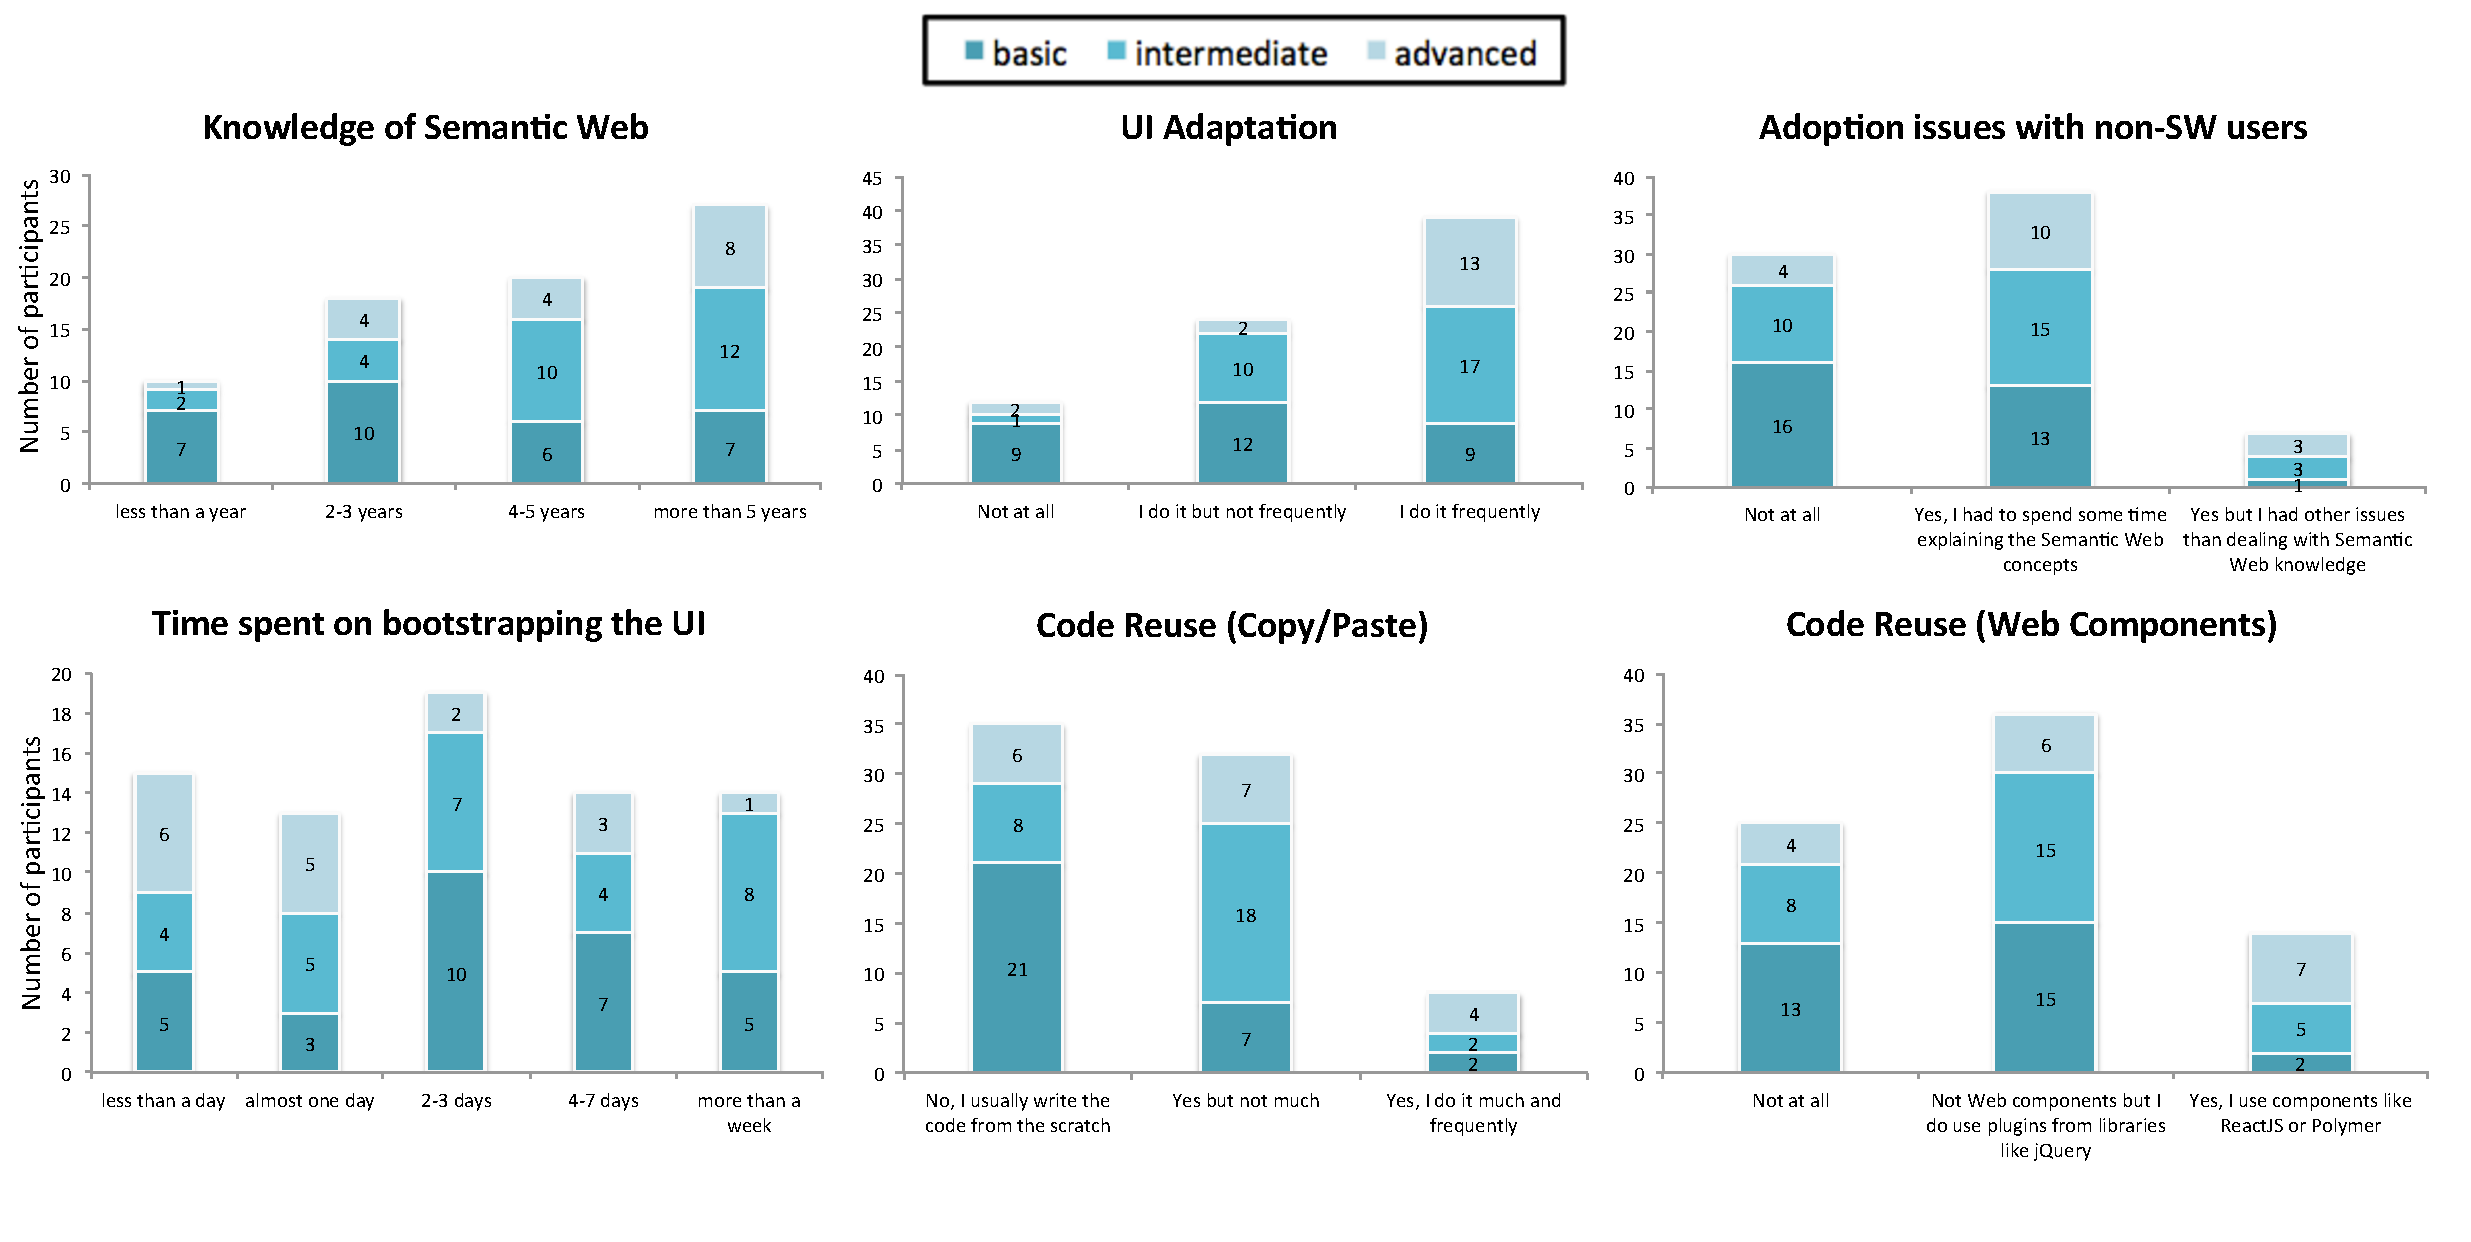
\includegraphics[width=1\linewidth]{images/userstudy.pdf}
  \caption{Results of our user study on the current status of LDA UI development.}
  \label{fig:userstudy}
\end{figure*}

\section{The Current Status of Linked Data User Interface Development}
In order to understand the current pitfalls of LDA UI design, we conducted a survey targeting %\textbf{75}
active Semantic Web developers\footnote{results are available at \url{https://goo.gl/cltqhv}}.
The participants where selected from the community of Semantic Web developers on Github who have had at least one active Semantic Web-related repository.
Github is currently the most popular repository for open source code and its transparent environment implies a suitable basis for evaluating reuse and collaboration among developers~\cite{Lima14,Tsay2014}.
We used Github APIs\footnote{\url{https://developer.github.com/v3/}} to search\footnote{keywords: "Semantic Web" OR "Linked Data" OR "RDF" OR "SPARQL"} for the potential Semantic Web repositories and then to collect the contact information of the corresponding contributors when available.
The search, after removing the organizations and invalid email addresses, resulted in 650 potential Semantic Web developers.
We then contacted the potential candidates to ask them about the current pitfalls in developing LDA UIs.
In our enquiry, we clearly mentioned to skip the questionnaire if they have not developed any Semantic Web application so far.
We used a minimal set of 7 questions to attract more responses and also used inline forms for GMail users to allow filling out the questionnaire in the same time as reading the enquiry email.
We collected 75 responses to our questionnaire, which is a considerable number of participants (almost 11.5\% of the potential candidates).
%The number of participants who filled in our questionnaire at the end was 75 (almost 11.5\% of the potential candidates which is still a considerable number of participants).
\autoref{fig:userstudy} shows the main results of our survey.

\paragraph{Participants}
Based on their LDA development experience, we divided the participants into three groups: basic (less than 2 applications), intermediate (3-5 applications) and advanced (more than 5 applications) developers.
The result showed that the majority (60\%) of participants were intermediate and advanced developers.
In addition to the development experience, developers were asked about their knowledge of Semantic Web to compare their practical and conceptual experience.
As results revealed, the majority of participants (63\%) had proficient (4-5 years) and expert (more than 5 years) knowledge of Semantic Web and Linked Data which makes a good sample for our evaluation. 


Questions addressed the following topics:
\begin{itemize}

\item
\emph{Amount of time spent on bootstrapping LDA UIs.}
Before designing the UIs in an LDA, developers need to spend some time on creating the skeleton of their application where querying data and the business logic of the application is handled.
The results confirm that developers spend a lot of time (on average more than 2 days) on bootstrapping their LDAs before they can start working on the UI.
 
\item
\emph{Reuse of code by Semantic Web developers.}
Developers usually reuse sections of code, templates, functions, and objects to save time and resources when developing LDAs.
We asked participants about two types of reuse: reuse by copy/pasting code from existing LDAs and reuse by employing current Web components.
Reuse by copy/pasting code can be an indicator on the standardization, modularity and reusability of current LDAs.
The results indicate that a considerable amount of users (46\%), prefer to write the code from the scratch instead of reusing the code from the existing Semantic Web projects.
This situation is more pronounced for basic developers who still prefer to write the code from the scratch although they have less experience in programming LDAs.
Furthermore, the results on reuse of Web components give an insight on the adoption of current Web Components by Semantic Web developers.
The results indicate that despite the prevalence of Web Components solutions, only 19\% of the participants (mainly advanced users) were employing them in their applications.
Interestingly, the majority of participants (49\%) were already reusing other component-like libraries which shows an attitude and capacity towards adopting the Web components.

\item
\emph{Adaptation of LDA UIs.}
Most of the modern Web applications provide a mechanism to customize and personalize their user interfaces based on the type of data and the information needs of their end users.
Proactive user interface adaptation allows the application to act more like a human and consequently, more intelligently~\cite{adaptiveSW2011}. 
As our study shows, within the current LDA developers, 52\% had experience adapting the user interface of their applications frequently. There were also 32\% that were doing the UI adaptation but not frequently.

\item
\emph{Adoption issues with non-Semantic Web developers.}
In order to examine if there is a communication gap between UI designers and Semantic Web developers, we asked the participants about their experience when collaborating with a non-SW developer.
Among the participants, 51\% had communication issues with non-Semantic Web developers to familiarize them with Semantic Web concepts before they can start contributing to the application.
The distribution of this issue among more experienced developers (45\% of the intermediate and advanced users) further emphasizes the importance of this communication gap.

\end{itemize}

\section{Adaptive Linked Data-driven Web Components}
In order to streamline the process of UI development in LDAs, we propose an architecture of adaptive LD-R Web components -- Web components enriched by the RDF data model.
As shown in \autoref{fig:framework}, the proposed architecture addresses LDA UI reusability and flexibility by incorporating RDF-based Web components and scopes.
In the following sections, the main elements of the architecture are described:

\subsection{LD-R Web Components}
As depicted in \autoref{fig:architecture}, there are 4 core component levels in an LD-R Web application.
Each core component abstracts the actions required for retrieving and updating the graph-based data and provides a basis for user-defined components to interact with Linked Data in three modes: view, edit and browse.
%For example, a viewer in the level of \emph{Dataset} component can enable visualizing a set of resources based on a certain property value whereas a viewer in the level of \emph{Resource} component can only allow visualizing properties of a specific resource (or a specific type of resource).

\begin{figure}[htb]
	\center
  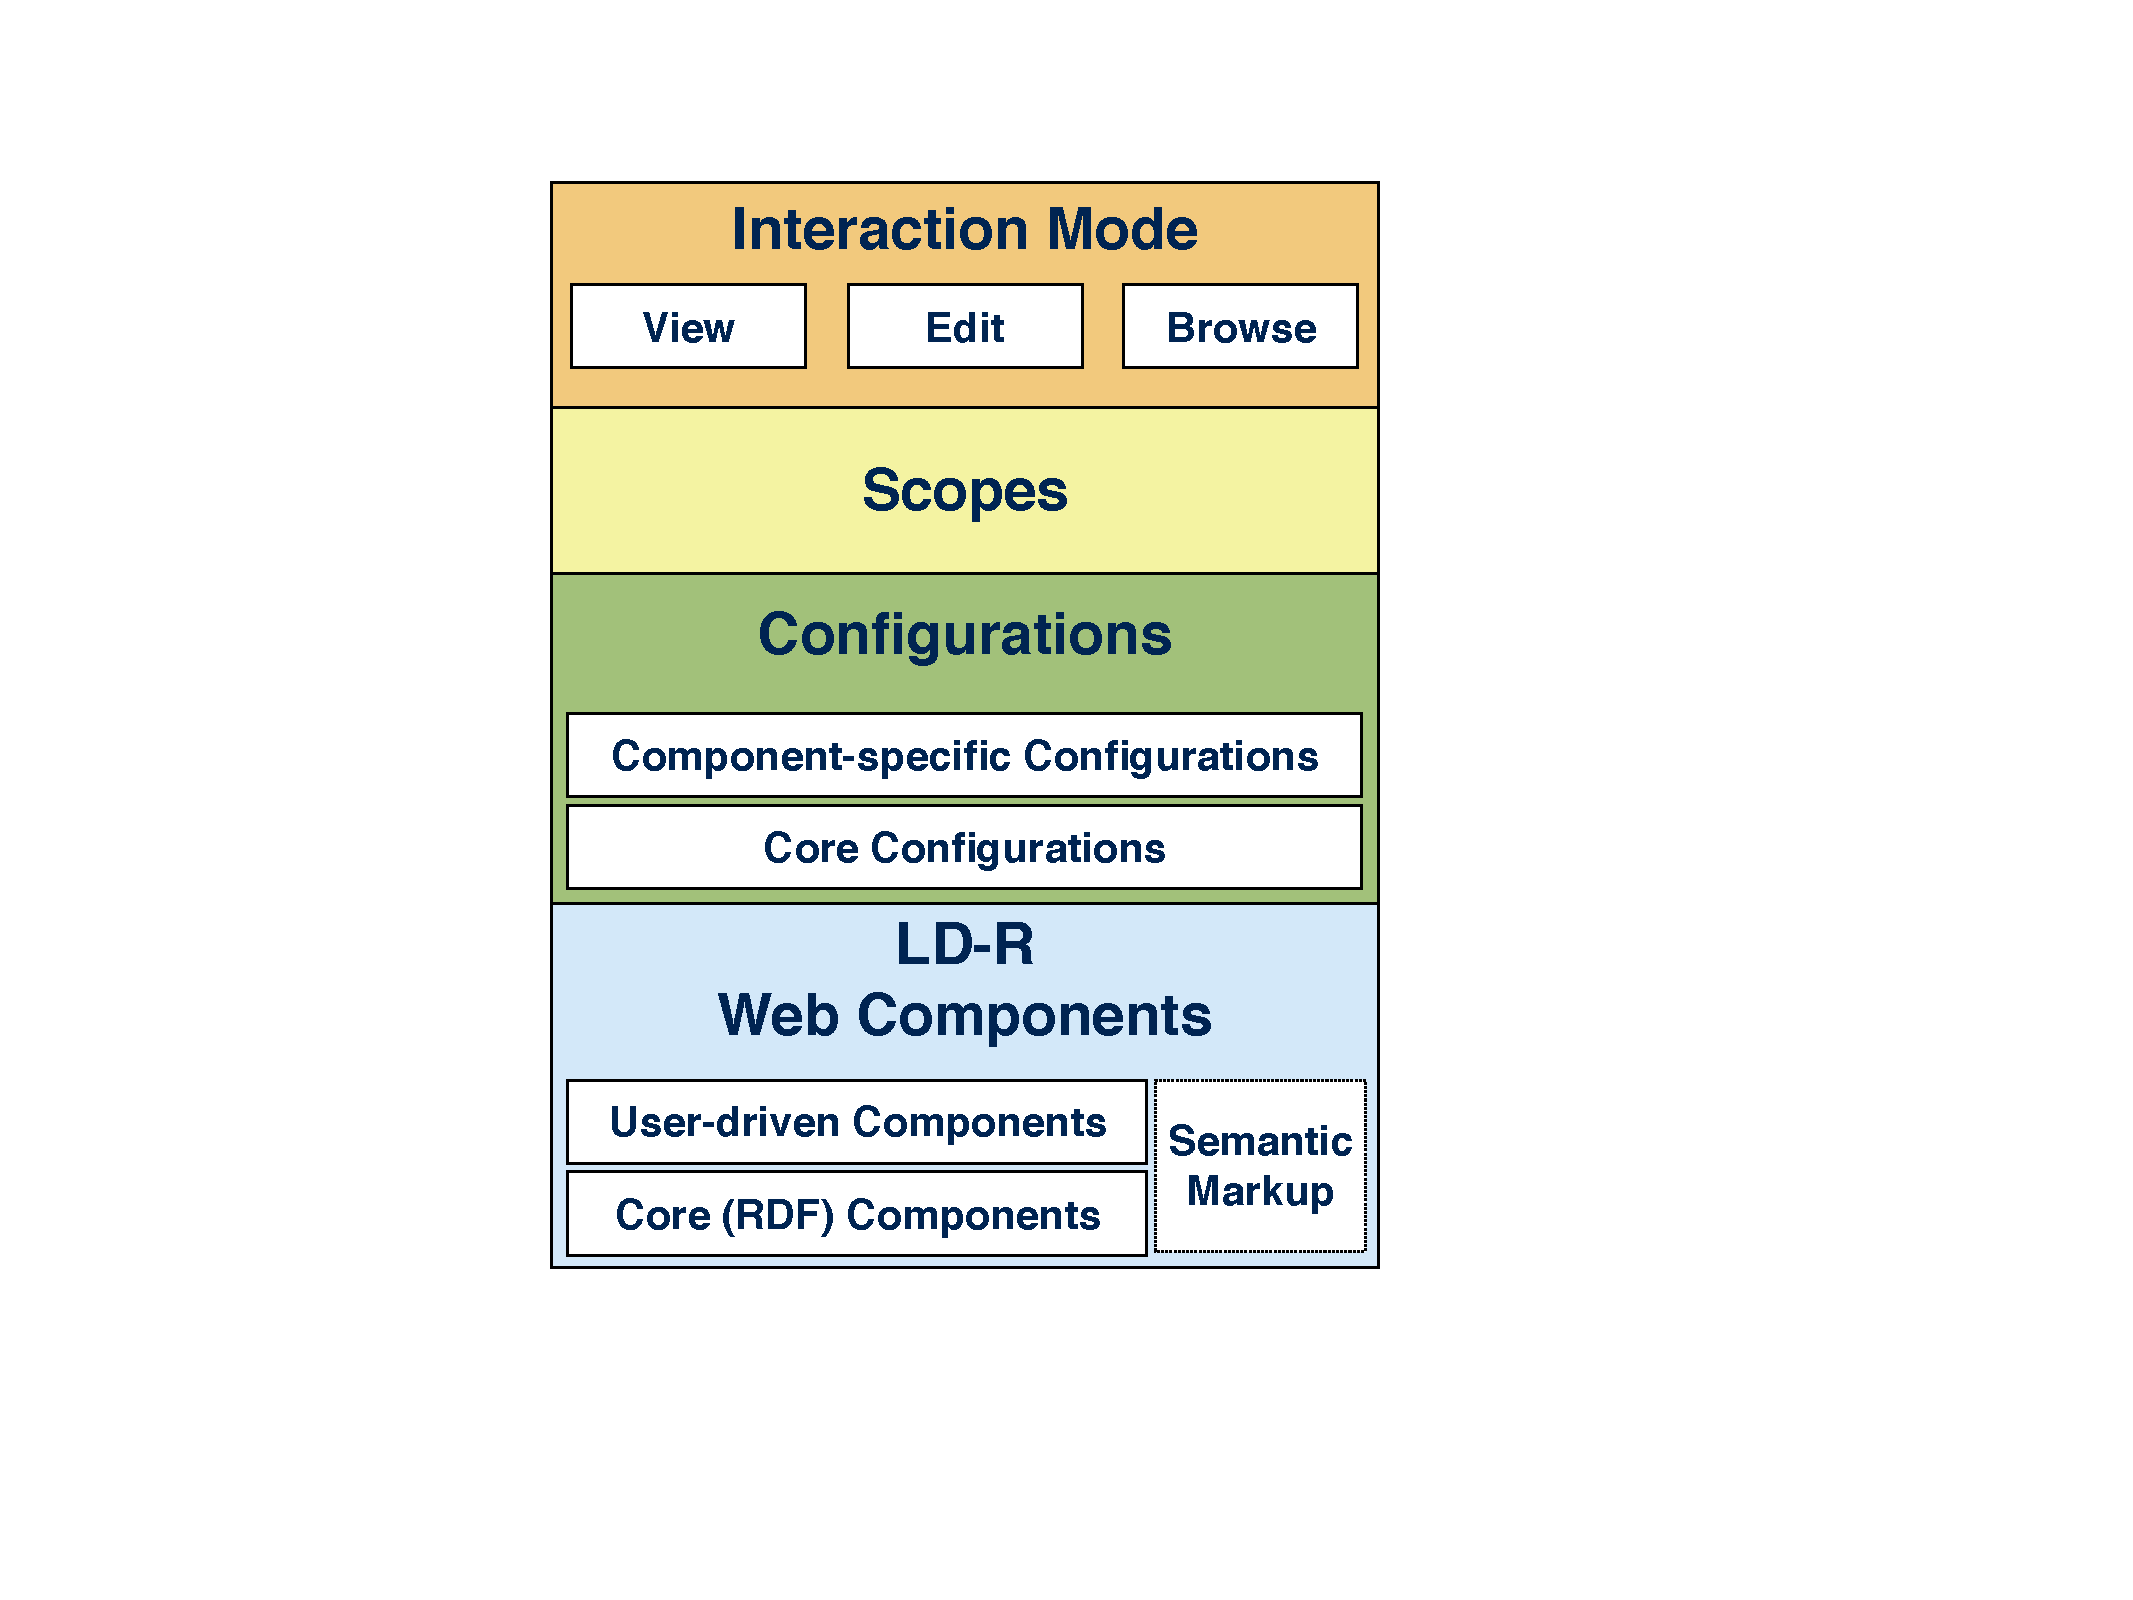
\includegraphics[width=0.80\linewidth]{images/framework.pdf}
  \caption{Main elements of the adaptive LD-R Web components architecture.}
  \label{fig:framework}
\end{figure}

\begin{figure}[htb]
  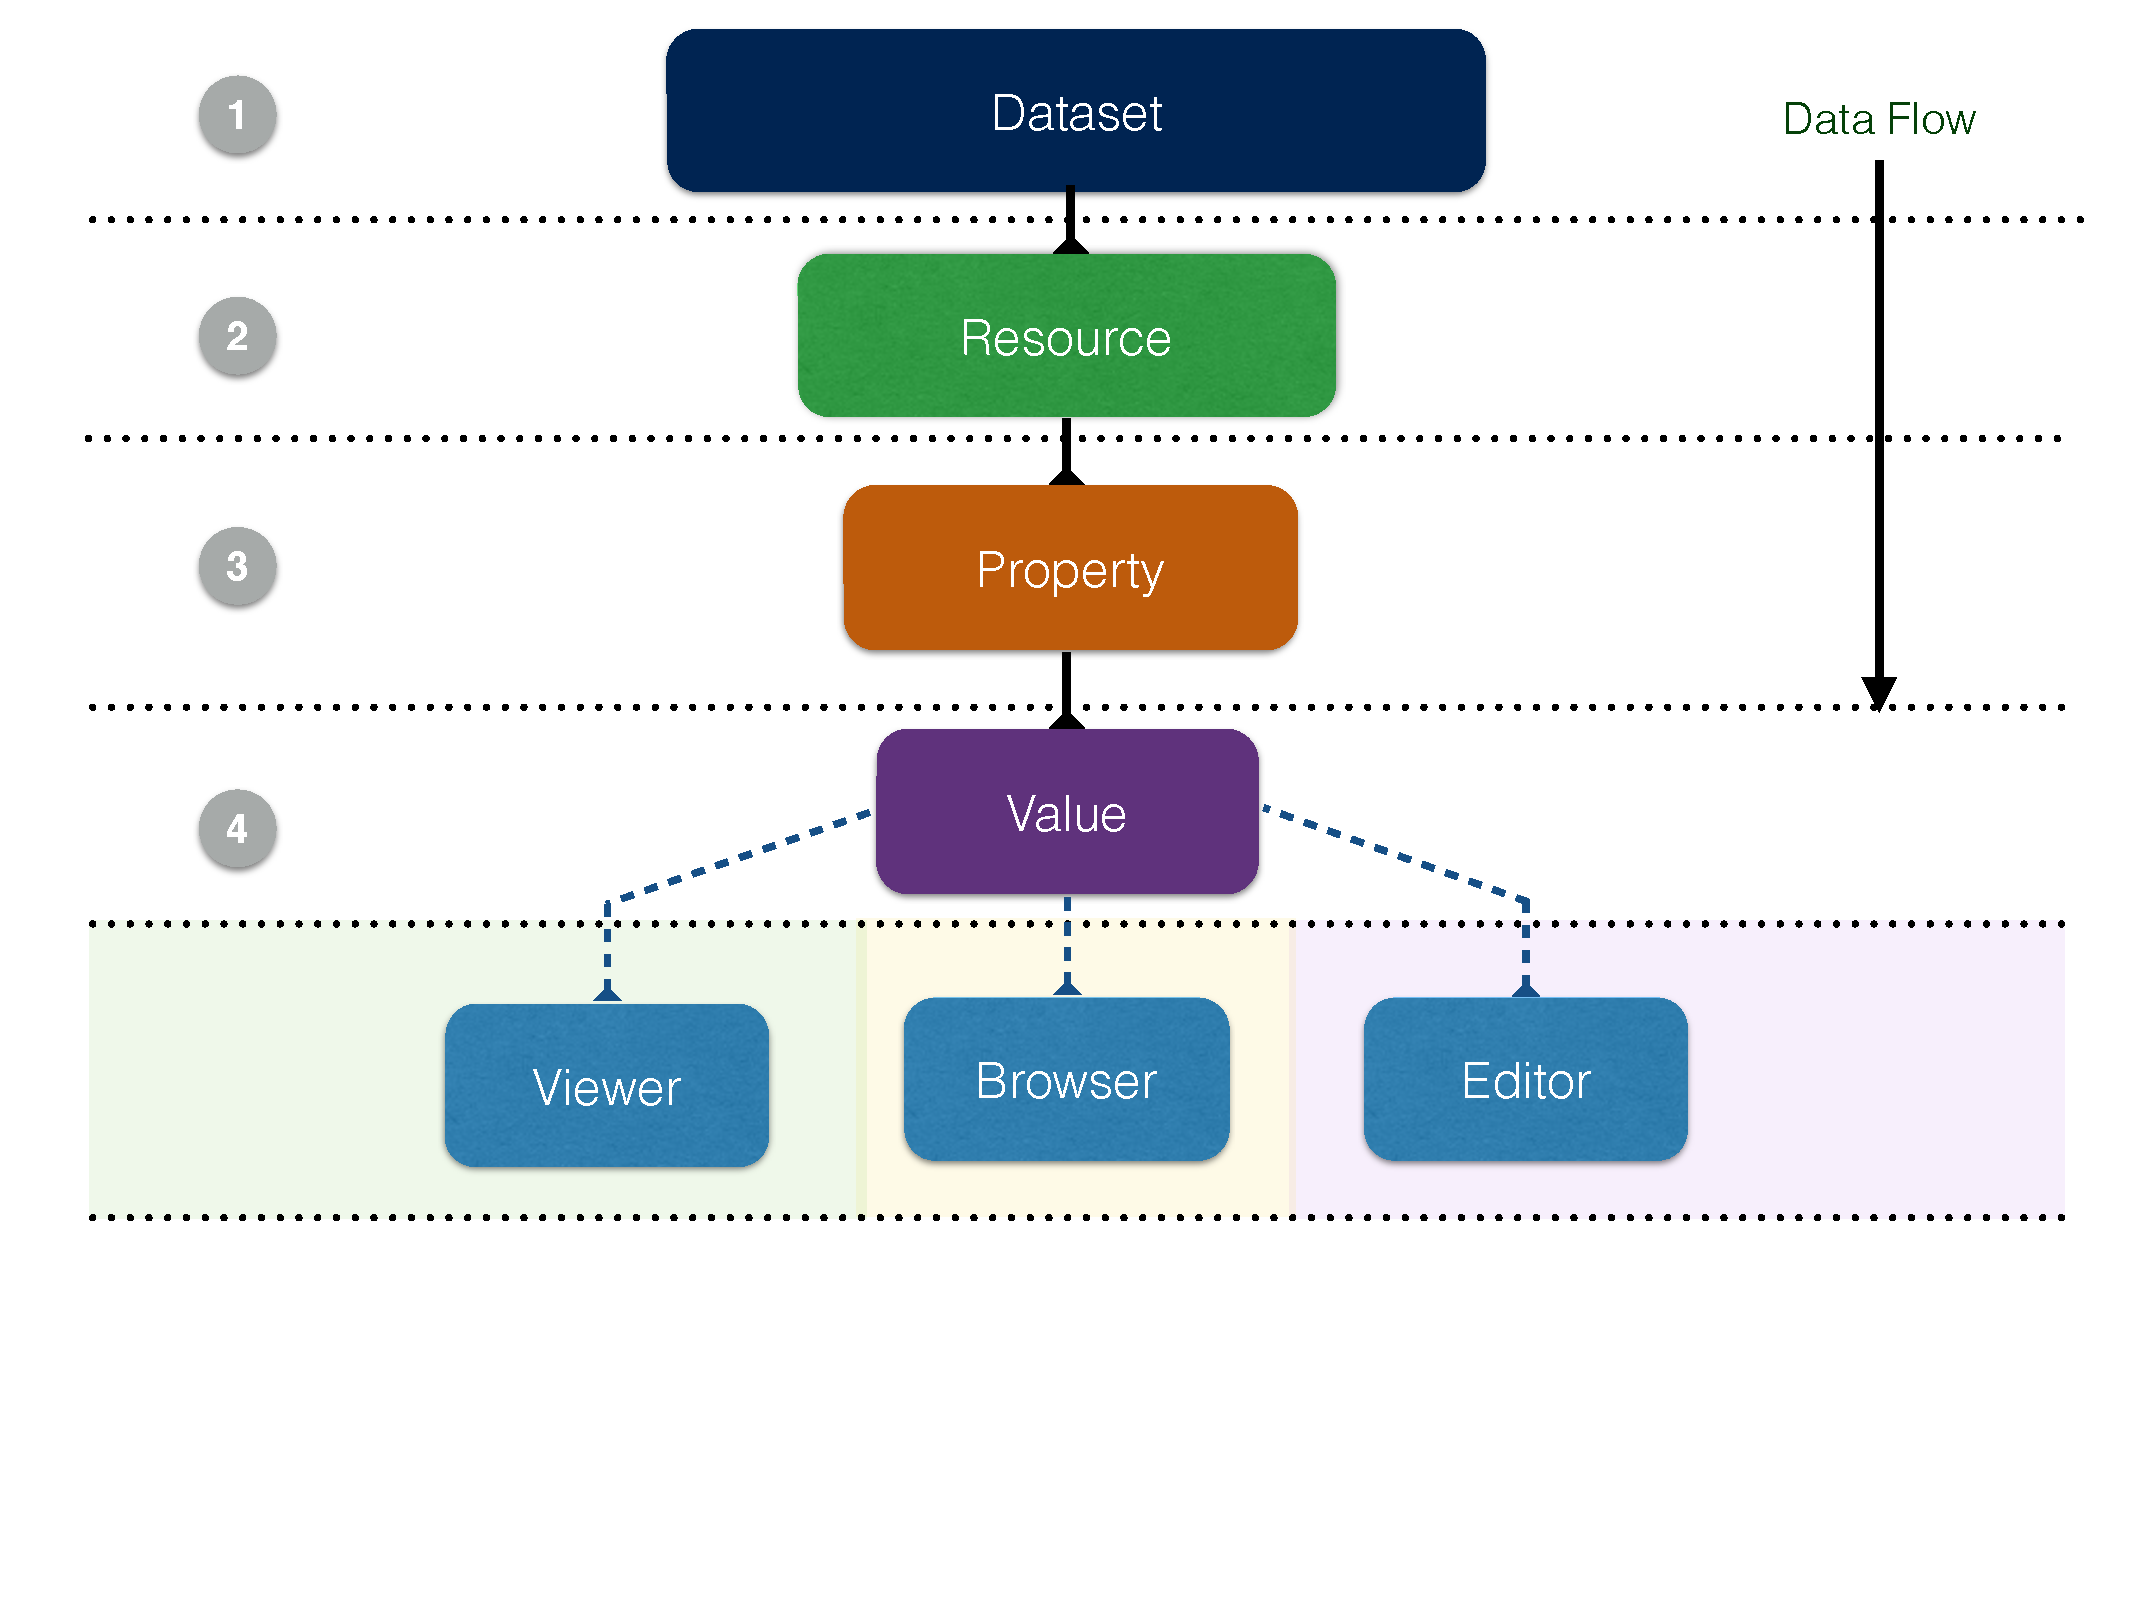
\includegraphics[width=1\linewidth]{images/architecture.pdf}
  \caption{Core LD-R Web components.}
  \label{fig:architecture}
\end{figure}

The data-flow in the system starts from the \emph{Dataset} component which handles all the events related to a set of resources under a named graph identified using a URI.
The next level is the \emph{Resource} component which is identified by a URI and indicates what is described in the application.
A resource is described by a set of properties which are handled by the \emph{Property} component. 
Properties can be either individual or aggregate when combining multiple features of a resource (e.g. a component that combines longitude and latitude properties; start date and end date properties for a date range, etc.).
Each property is instantiated by an individual value or multiple values in case of an aggregate object. 
The value(s) of properties are controlled by the \emph{Value} component.
In turn, Value components invoke different components to view, edit and browse the property values.
\emph{Viewer}, \emph{Editor} and \emph{Browser} components are terminals in the LD-R single directional data flow where customized user-generated components can be plugged into the system.
These components apply on individual and aggregate values (e.g. to show multiple coordinates on a map).

\subsection{Scopes and Configurations}

\begin{figure}[tb]
  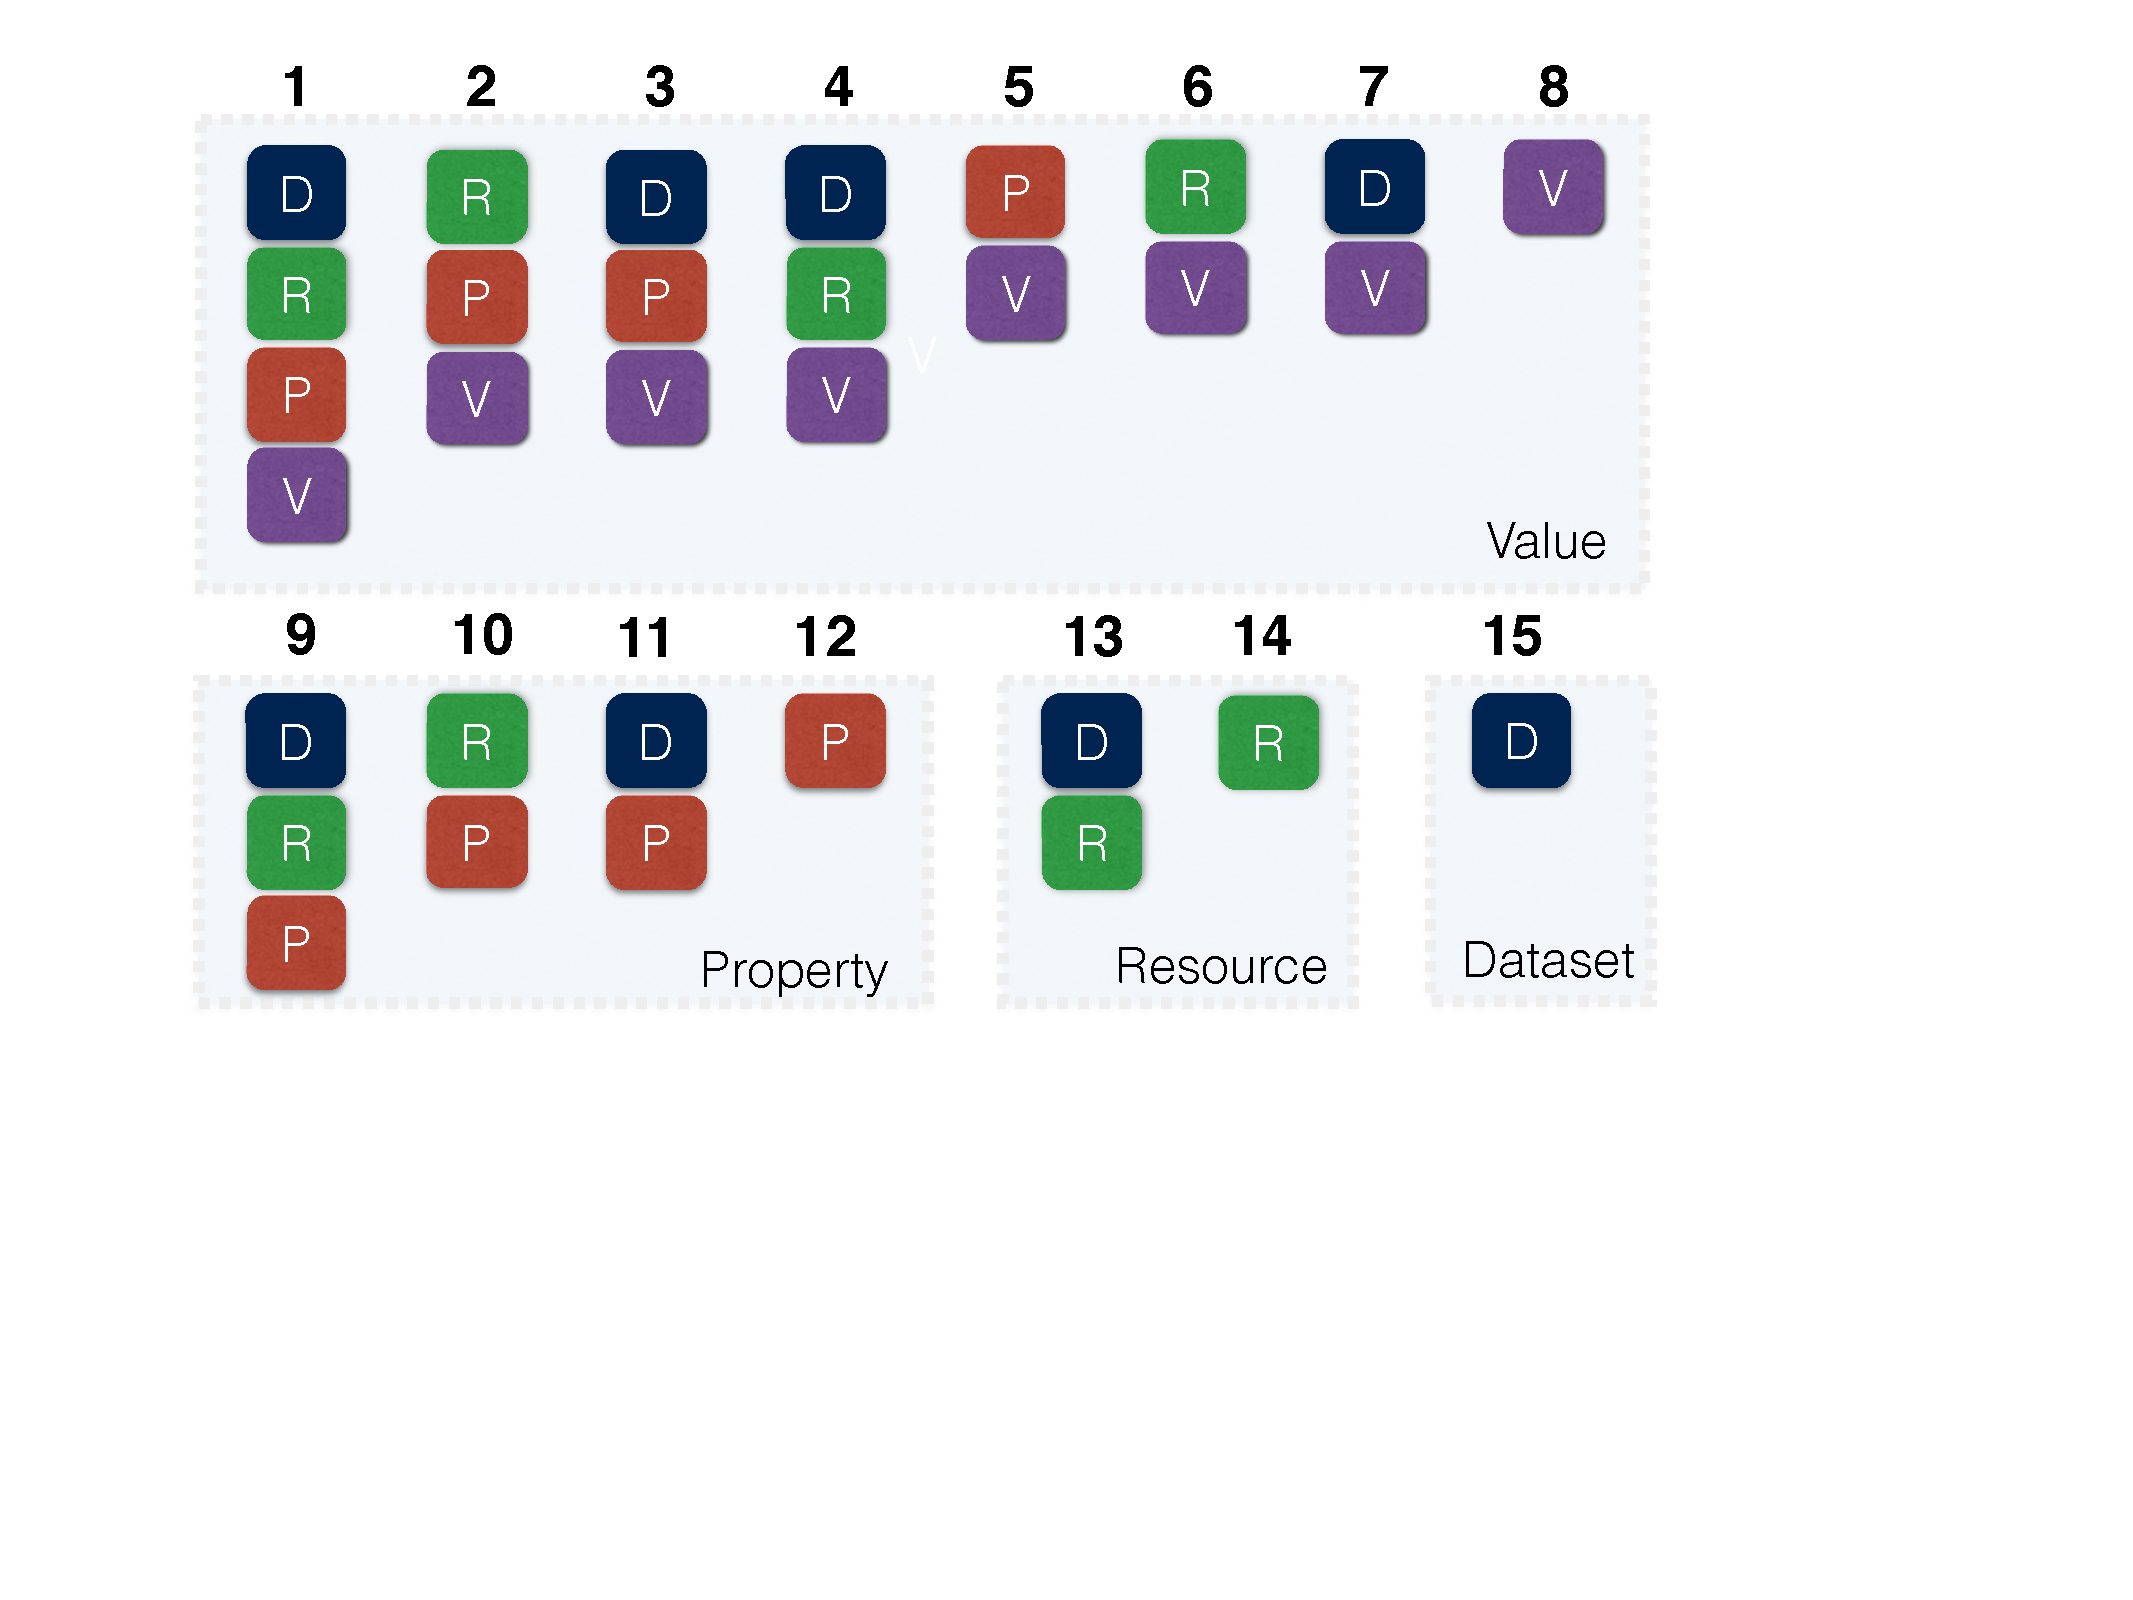
\includegraphics[width=.95\linewidth]{images/scopes.pdf}
  \caption{LD-R scopes based on the permutation of dataset, resource, property and value identifiers.}
  \label{fig:scopes}
\end{figure}

\begin{figure}[tb]
 \center
  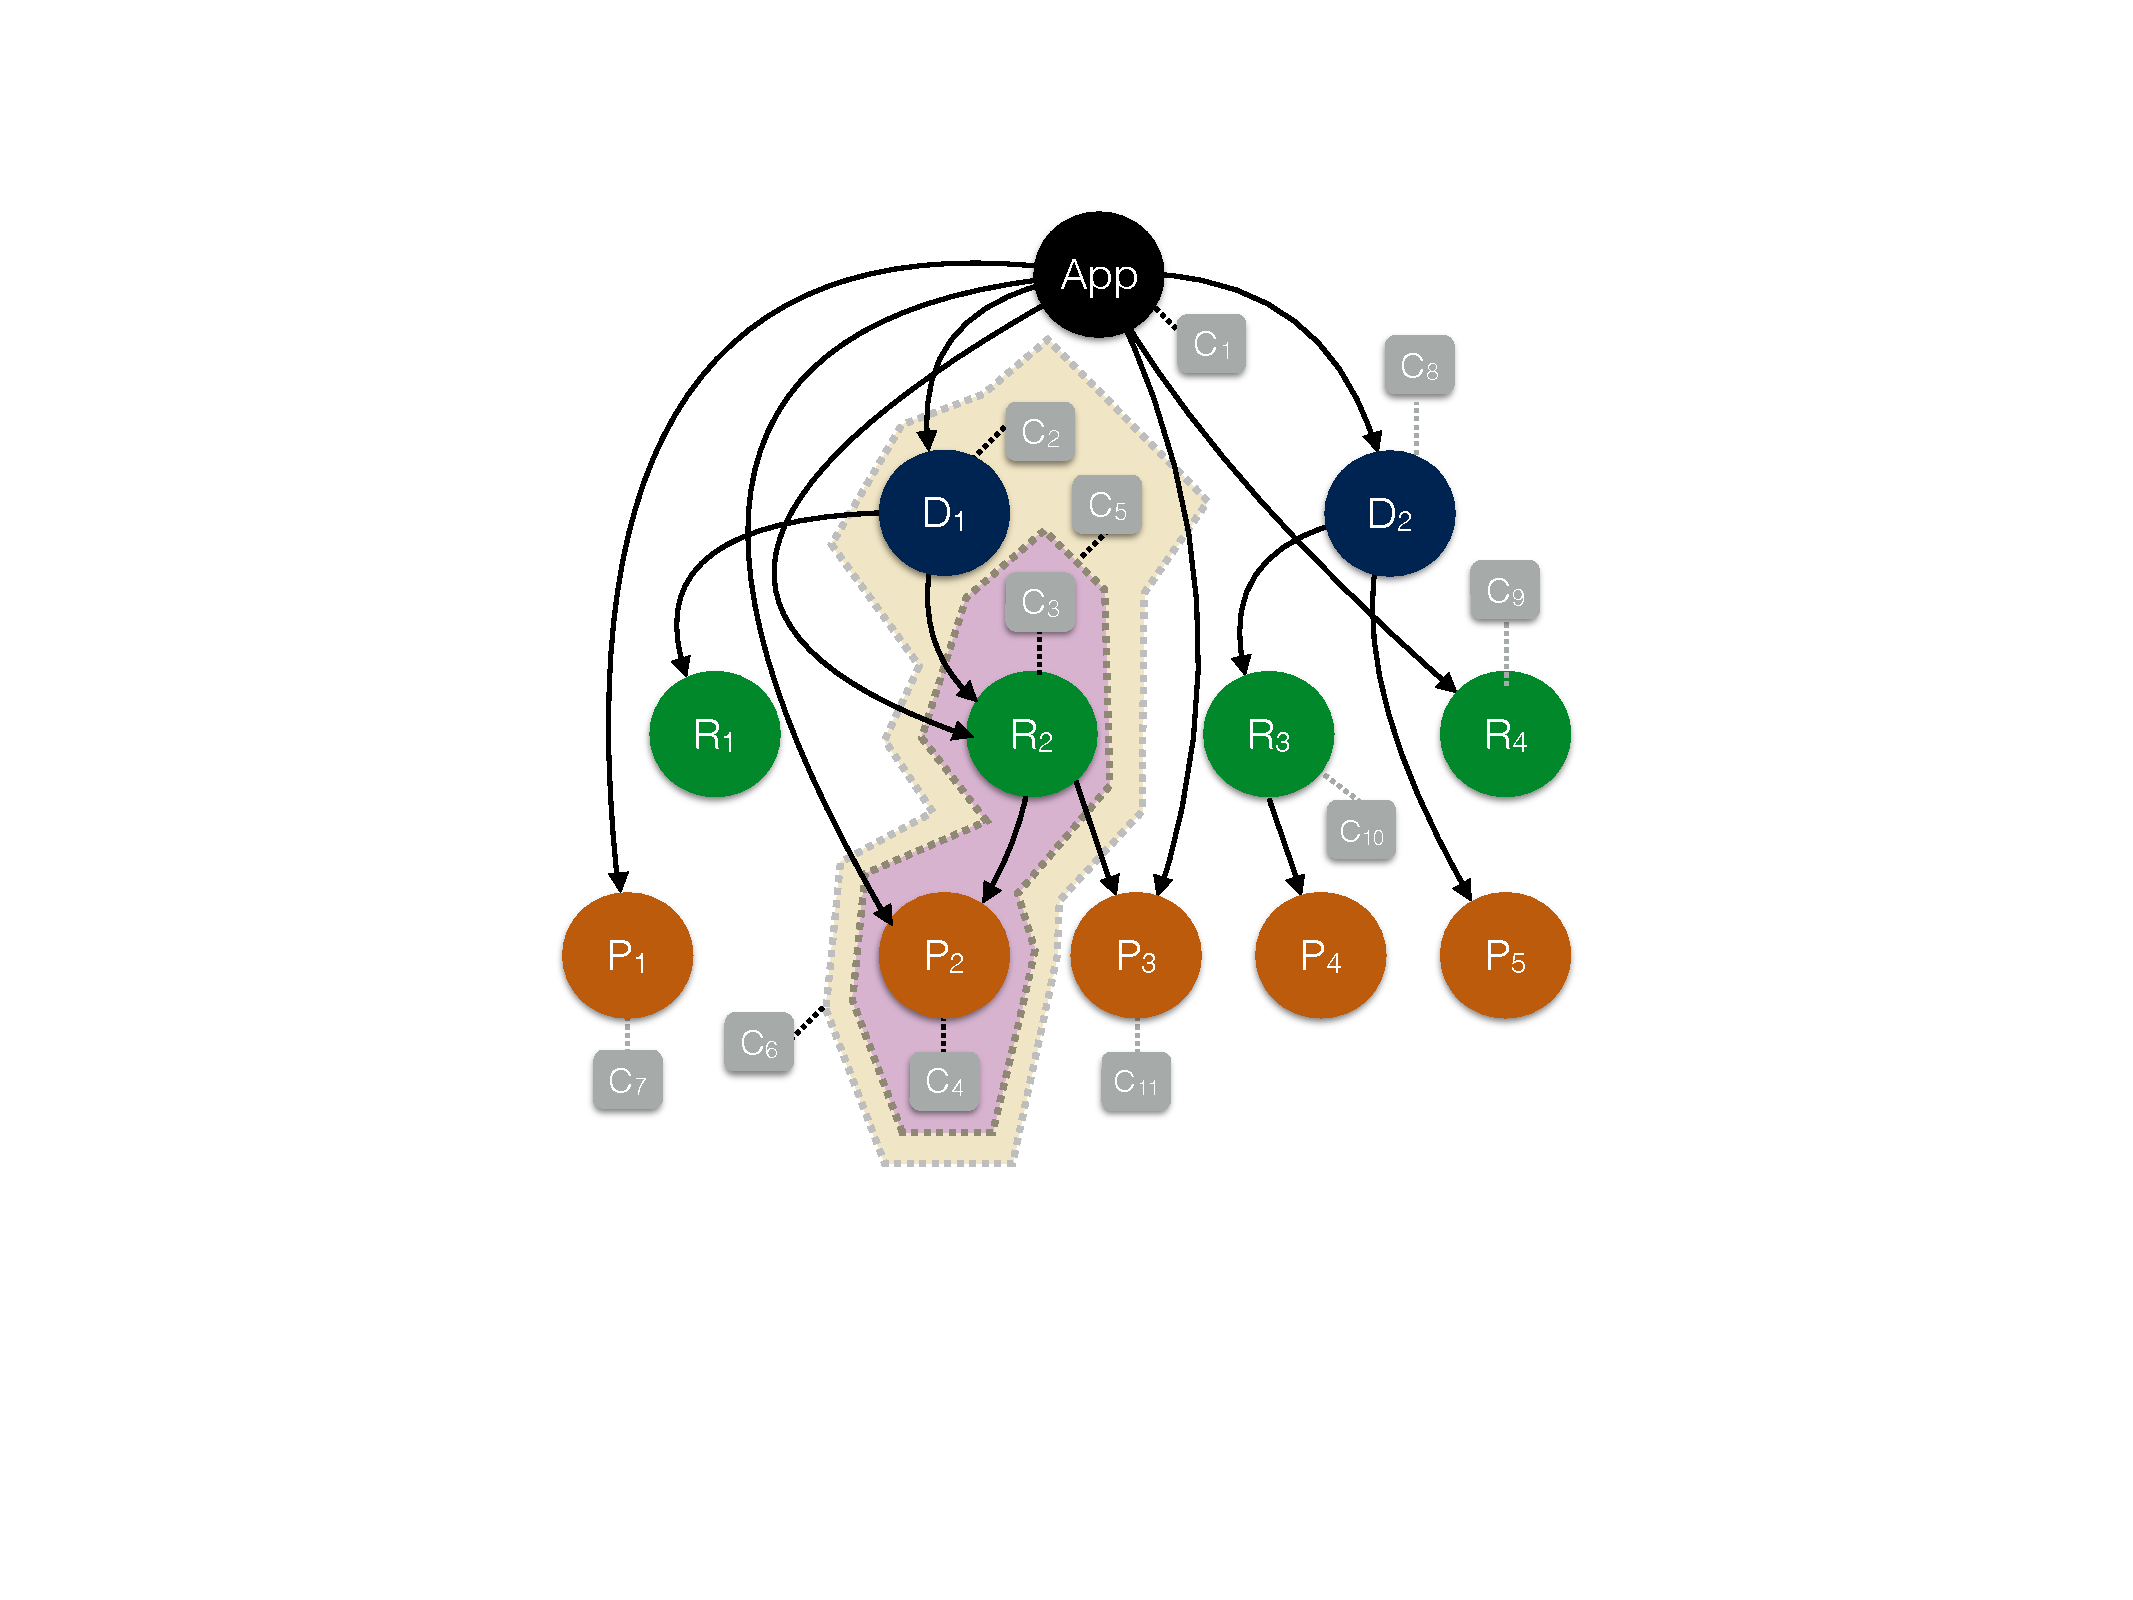
\includegraphics[width=.73\linewidth]{images/exampleConfig.pdf}
  \caption{A sample LD-R configuration hypergraph.}
  \label{fig:exampleConfig}
\end{figure}

LD-R Web components provide a versatile approach for context adaptation.
A context can be a specific domain of interest, a specific user requirement or both.
In order to enable customization and personalization, the LD-R approach exploits the concepts of \emph{Scope} and \emph{Configuration}.
A scope is defined as a hierarchical permutation of Dataset, Resource, Property and Value components (cf. \autoref{fig:scopes}).
Each scope conveys a certain level of specificity on a given context ranging from 1 (most specific) to 15 (least specific).
Scopes are defined by using either the URIs of named graphs, resources and properties, or by identifying the resource types and data types.
A configuration is defined as a setting which affects the way the LDA and Web components are interpreted and rendered (e.g. enforce a component to display Wikipedia page URIs for DBpedia resources).
UI adaptation is handled by traversing the configurations for scopes, populating the configurations and overwriting the configurations when a more specific applicable scope is found:

\begin{lstlisting}[firstnumber=1, backgroundcolor=\color{white}, basicstyle=\small\tt, label=code:adaptation, caption=Algorithm for the LD-R UI adaptation.]
InitialConfig = {initial application configuration}
Context = [array of scopes with the corresponding configuration objects]
Config = InitialConfig
for (i = 15; i < 1; i--) {
    Config.compareWith(Context[i]) {
        Config.addMissingAttributes()
        Config.overwriteExistingAttributes()
    }
}
\end{lstlisting}

\autoref{fig:exampleConfig} demonstrates an example of the LD-R configuration hypergraph containing scopes with the maximum depth of \texttt{DRP}.
The graph defines a generic configuration for the application as C$_{\text{1}}$.
There are configurations defined for the dataset scope D$_{\text{1}}$ as C$_{\text{2}}$, for the resource scope R$_{\text{2}}$ as C$_{\text{3}}$ and for the property scope P$_{\text{2}}$ as C$_{\text{4}}$.
There are also configurations for the \texttt{RP} scope R$_{\text{2}}$P$_{\text{2}}$ as C$_{\text{5}}$ and for the \texttt{DRP} scope D$_{\text{1}}$R$_{\text{2}}$P$_{\text{2}}$ as C$_{\text{6}}$.
Let's suppose we have a setting with the following values for the scopes and configurations:
\begin{compactitem}

\item
D$_{\text{1}}$= \texttt{<http://ld-r.org/users>}
\item
R$_{\text{2}}$= type \texttt{foaf:Person}
\item
P$_{\text{2}}$= \texttt{rdfs:label}
\item
C$_{\text{1}}$=\{\{viewer:`basic'\},\{attr$_{\text{1}}$:1\},\{attr$_{\text{2}}$:3\}\}
\item
C$_{\text{2}}$=\{\{attr$_{\text{1}}$:0\},\{attr$_{\text{3}}$:2\}\}
\item
C$_{\text{3}}$=\{\{attr$_{\text{3}}$:1\},\{attr$_{\text{4}}$:4\},\{attr$_{\text{5}}$:1\}\}
\item
C$_{\text{4}}$=\{\{attr$_{\text{5}}$:2\},\{attr$_{\text{6}}$:1\}\}
\item
C$_{\text{5}}$=\{\{viewer:`contact'\},\{attr$_{\text{3}}$:5\},\{attr$_{\text{7}}$:6\}\}
\item
C$_{\text{6}}$=\{\{attr$_{\text{3}}$:8\},\{attr$_{\text{7}}$:1\},\{attr$_{\text{8}}$:3\}\}
\end{compactitem}

With the above settings, when a property component for \texttt{rdfs:label} is rendered without the dataset and resource context, the configuration will be:

 \{\{viewer:`basic'\},\{attr$_{\text{1}}$:1\},\{attr$_{\text{2}}$:3\},\{attr$_{\text{5}}$:2\},\{attr$_{\text{6}}$:1\}\} 
 
When the property component gets rendered within the resource context of type \texttt{foaf:Person}, the settings for viewer and attr$_{\text{5}}$ are overwritten and new settings for attr$_{\text{3}}$, attr$_{\text{4}}$ and attr$_{\text{7}}$ are added:

\{\{viewer:`contact'\},\{attr$_{\text{1}}$:1\},\{attr$_{\text{2}}$:3\},\{attr$_{\text{3}}$:5\},\{attr$_{\text{4}}$:4\},\\\{attr$_{\text{5}}$:1\},\{attr$_{\text{6}}$:1\},\{attr$_{\text{7}}$:6\}\} 

When the additional context of dataset as ~\texttt{<http://ld-r.org/users>} is given, attr$_{\text{3}}$ and attr$_{\text{7}}$ get overwritten and a new setting for attr$_{\text{8}}$ is added:

\{\{viewer:`contact'\},\{attr$_{\text{1}}$:0\},\{attr$_{\text{2}}$:3\},\{attr$_{\text{3}}$:8\},\{attr$_{\text{4}}$:4\},\\\{attr$_{\text{5}}$:1\},\{attr$_{\text{6}}$:1\},\{attr$_{\text{7}}$:1\},\{attr$_{\text{8}}$:3\}\} 
%and then for some specific properties \texttt{P} (e.g. \texttt{dcterms:title} or \texttt{rdfs:label}) within a specific resource (e.g. \texttt{<http://ld-r.org>}), we can change those configurations using the \texttt{RP} scope.
%Another example would be having a different rendering for all resources of a specific type (e.g. \texttt{foaf:Person}).

Scopes can also be defined on a per user basis, facilitating the versioning and reuse of user-specific configurations.
User-Specific configurations provide different views on components and thereby data, based on the different personas dealing with them.

In addition to the fine-grained component customization, LD-R Web applications provide a fine-grained access control over the data through the component scopes.
For example, an application developer can restrict access to a specific property of a specific resource in a certain dataset and on a specific interaction mode.

\subsection{Semantic Markup for Web Components}
\label{sec:markup}
The innate support of RDF in LD-R Web components enable the automatic creation of semantic markup in the UI level.
Lower semantic techniques such as \emph{RDFa}, \emph{Mircodata} and \emph{JSON-LD} can be incorporated in the core LD-R components to expose structured data to current search engines which are capable of parsing semantic markup.
For example, an LD-R component created based on the Good Relations\footnote{\url{http://www.heppnetz.de/projects/goodrelations/}} or \url{Schema.org} ontologies, can automatically expose the product data as Google Rich Snippets for products\footnote{\url{https://developers.google.com/structured-data/}} which will provide better visibility of the data on Web search results (i.e. SEO).

In addition to automatic annotation of data provided by the LD-R Web components, the approach offers semi-automatic markup of Web components by creating component metadata. 
Component metadata consists of two categories of markup:
\begin{itemize}
\item Automatic markup generated by parsing component package specification -- metadata about the component and its dependencies. It includes general metadata such as name, description, version, homepage, author as well as technical metadata on component source repository and dependencies.

\item Manual markup created by component authors which exposes metadata such as component level (dataset, resource, property, value), granularity (individual, aggregate), mode (view, edit, browse) and configuration parameters specification.

\end{itemize}

Similar to content markup, Component markup can utilize commonly-known ontologies such as \url{Schema.org} in order to improve the visibility of LD-R components and enable application assemblers to better understand the intended usage and capabilities of a given component.

\subsection{Stackeholders and Life Cycle}
\begin{figure}[tb]
  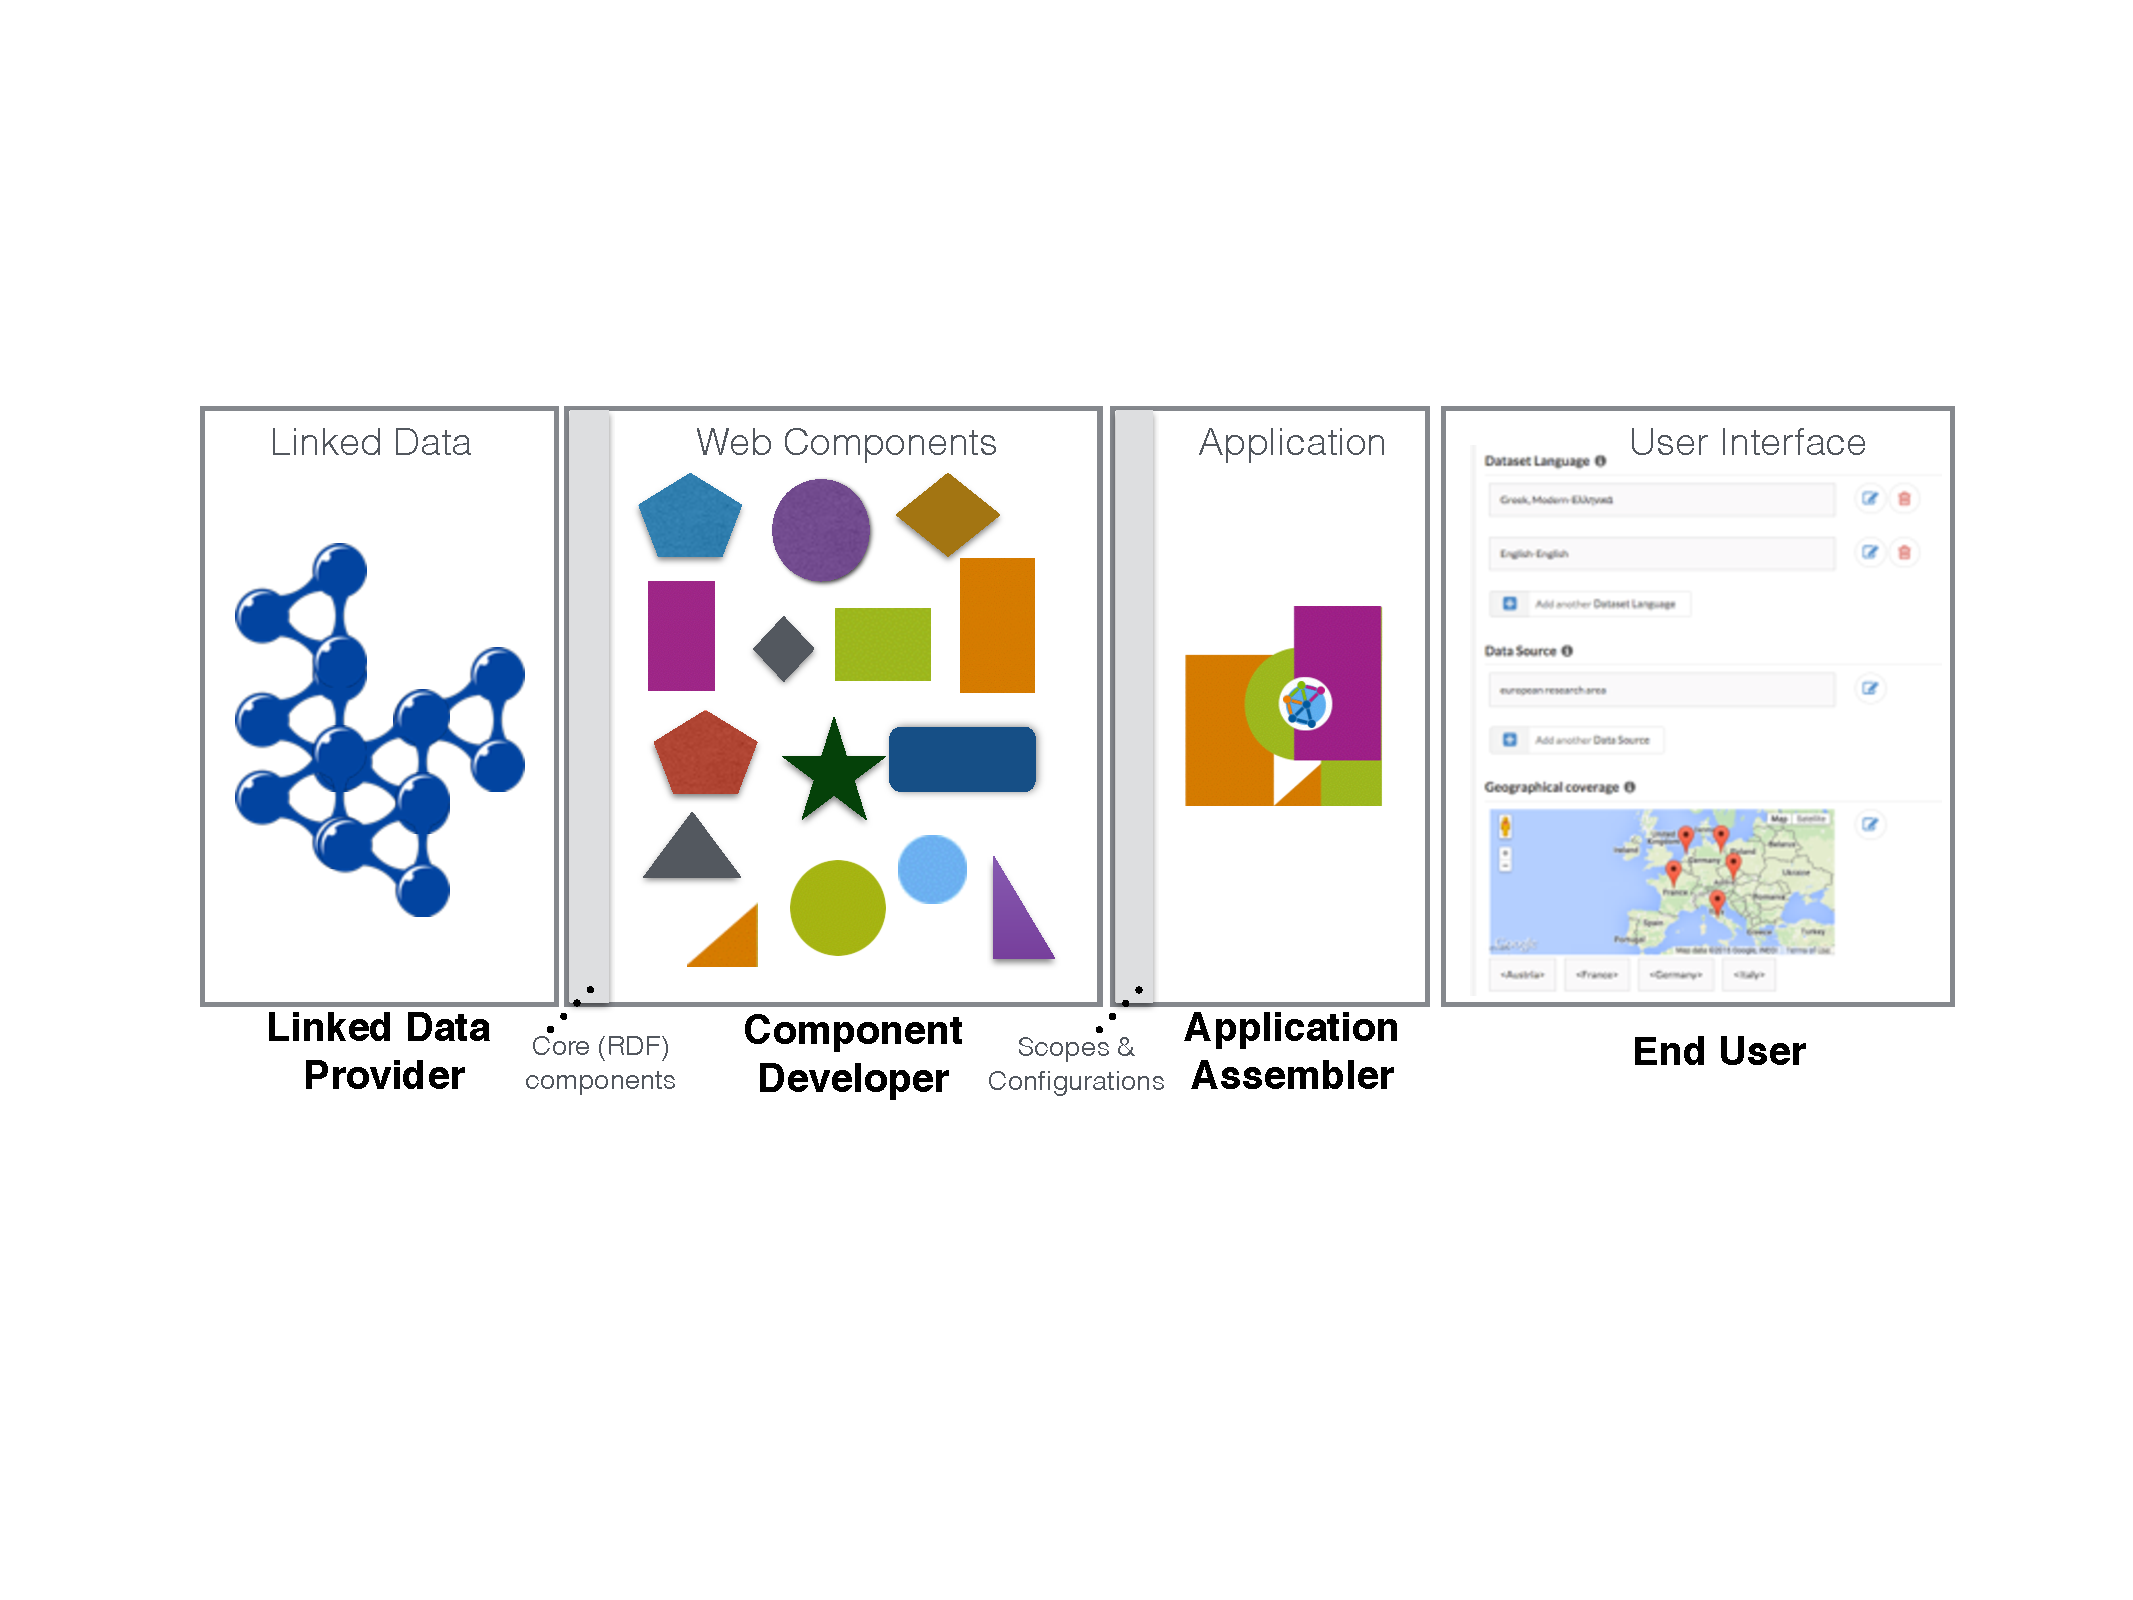
\includegraphics[width=1\linewidth]{images/lifecycle.pdf}
  \caption{LD-R components life cycle.}
  \label{fig:lifecycle}
\end{figure}

As shown in \autoref{fig:lifecycle}, the LD-R components lifecycle encompasses four primary types of stakeholders:

\begin{itemize}

\item \emph{Linked Data Provider}.
Since the LD-R approach focuses mainly on Linked Data applications, the provision of RDF-compliant data is an essential phase in developing the LD-R components.
There are different stages~\cite{AuerLOD2} in Linked Data provision, including data extraction, storage, interlinking, enrichment, quality analysis and repair which should be taken into account by data scientists and Linked Data experts.
Once the data and schemata are provided to the LD-R component system, the system can bring a reciprocal value to Linked Data providers to better understand and curate the data when needed.
For example, in the case of geo-coordinates, a map component can enable data providers to easily curate the outlier data (e.g. ambiguous entities) within a certain geo boundary in a visual manner.

\item \emph{Component Developer}. 
Component developers are UX designers and Web programmers who are involved in component fabrication.
There are two types of Web components developed in this step:
a) \emph{Core components} (cf. \autoref{fig:architecture}) which abstract the underlying RDF data model.
These components are built-in to the system, however can still be overwritten by developers who have proficiency in Semantic Web and Linked Data.
b) \emph{Community-driven components} which exploit the core components.
These components are either created from the scratch or by remixing and repurposing existing Web components found on the Web.

\item \emph{Application Assembler}.
The main task of application assembler is to identify the right components and configurations for the application; and to combine them in a way which fits the application requirement. 
Within the LD-R component system, the metadata provided by each Web component facilitates the discovery of relevant components.
Having shared vocabularies on Linked Open Data allows assemblers to not only reuse components but also reuse the existing configurations and scopes published on the Web.
For example, if there is already a suitable configuration for \texttt{RP} scope which uses \texttt{foaf:Person} as resource type and ~\texttt{dcterms:description} as property URI, the assembler can reuse that configuration within his application.

\item \emph{End User}. 
End users experience working with the components to pursue goals in a certain application domain.
As such, they may request the development of new components or configurations in order to fulfil their requirements and are expected to provide feedback on existing components.

\end{itemize}

\begin{figure}[tb]
\center
  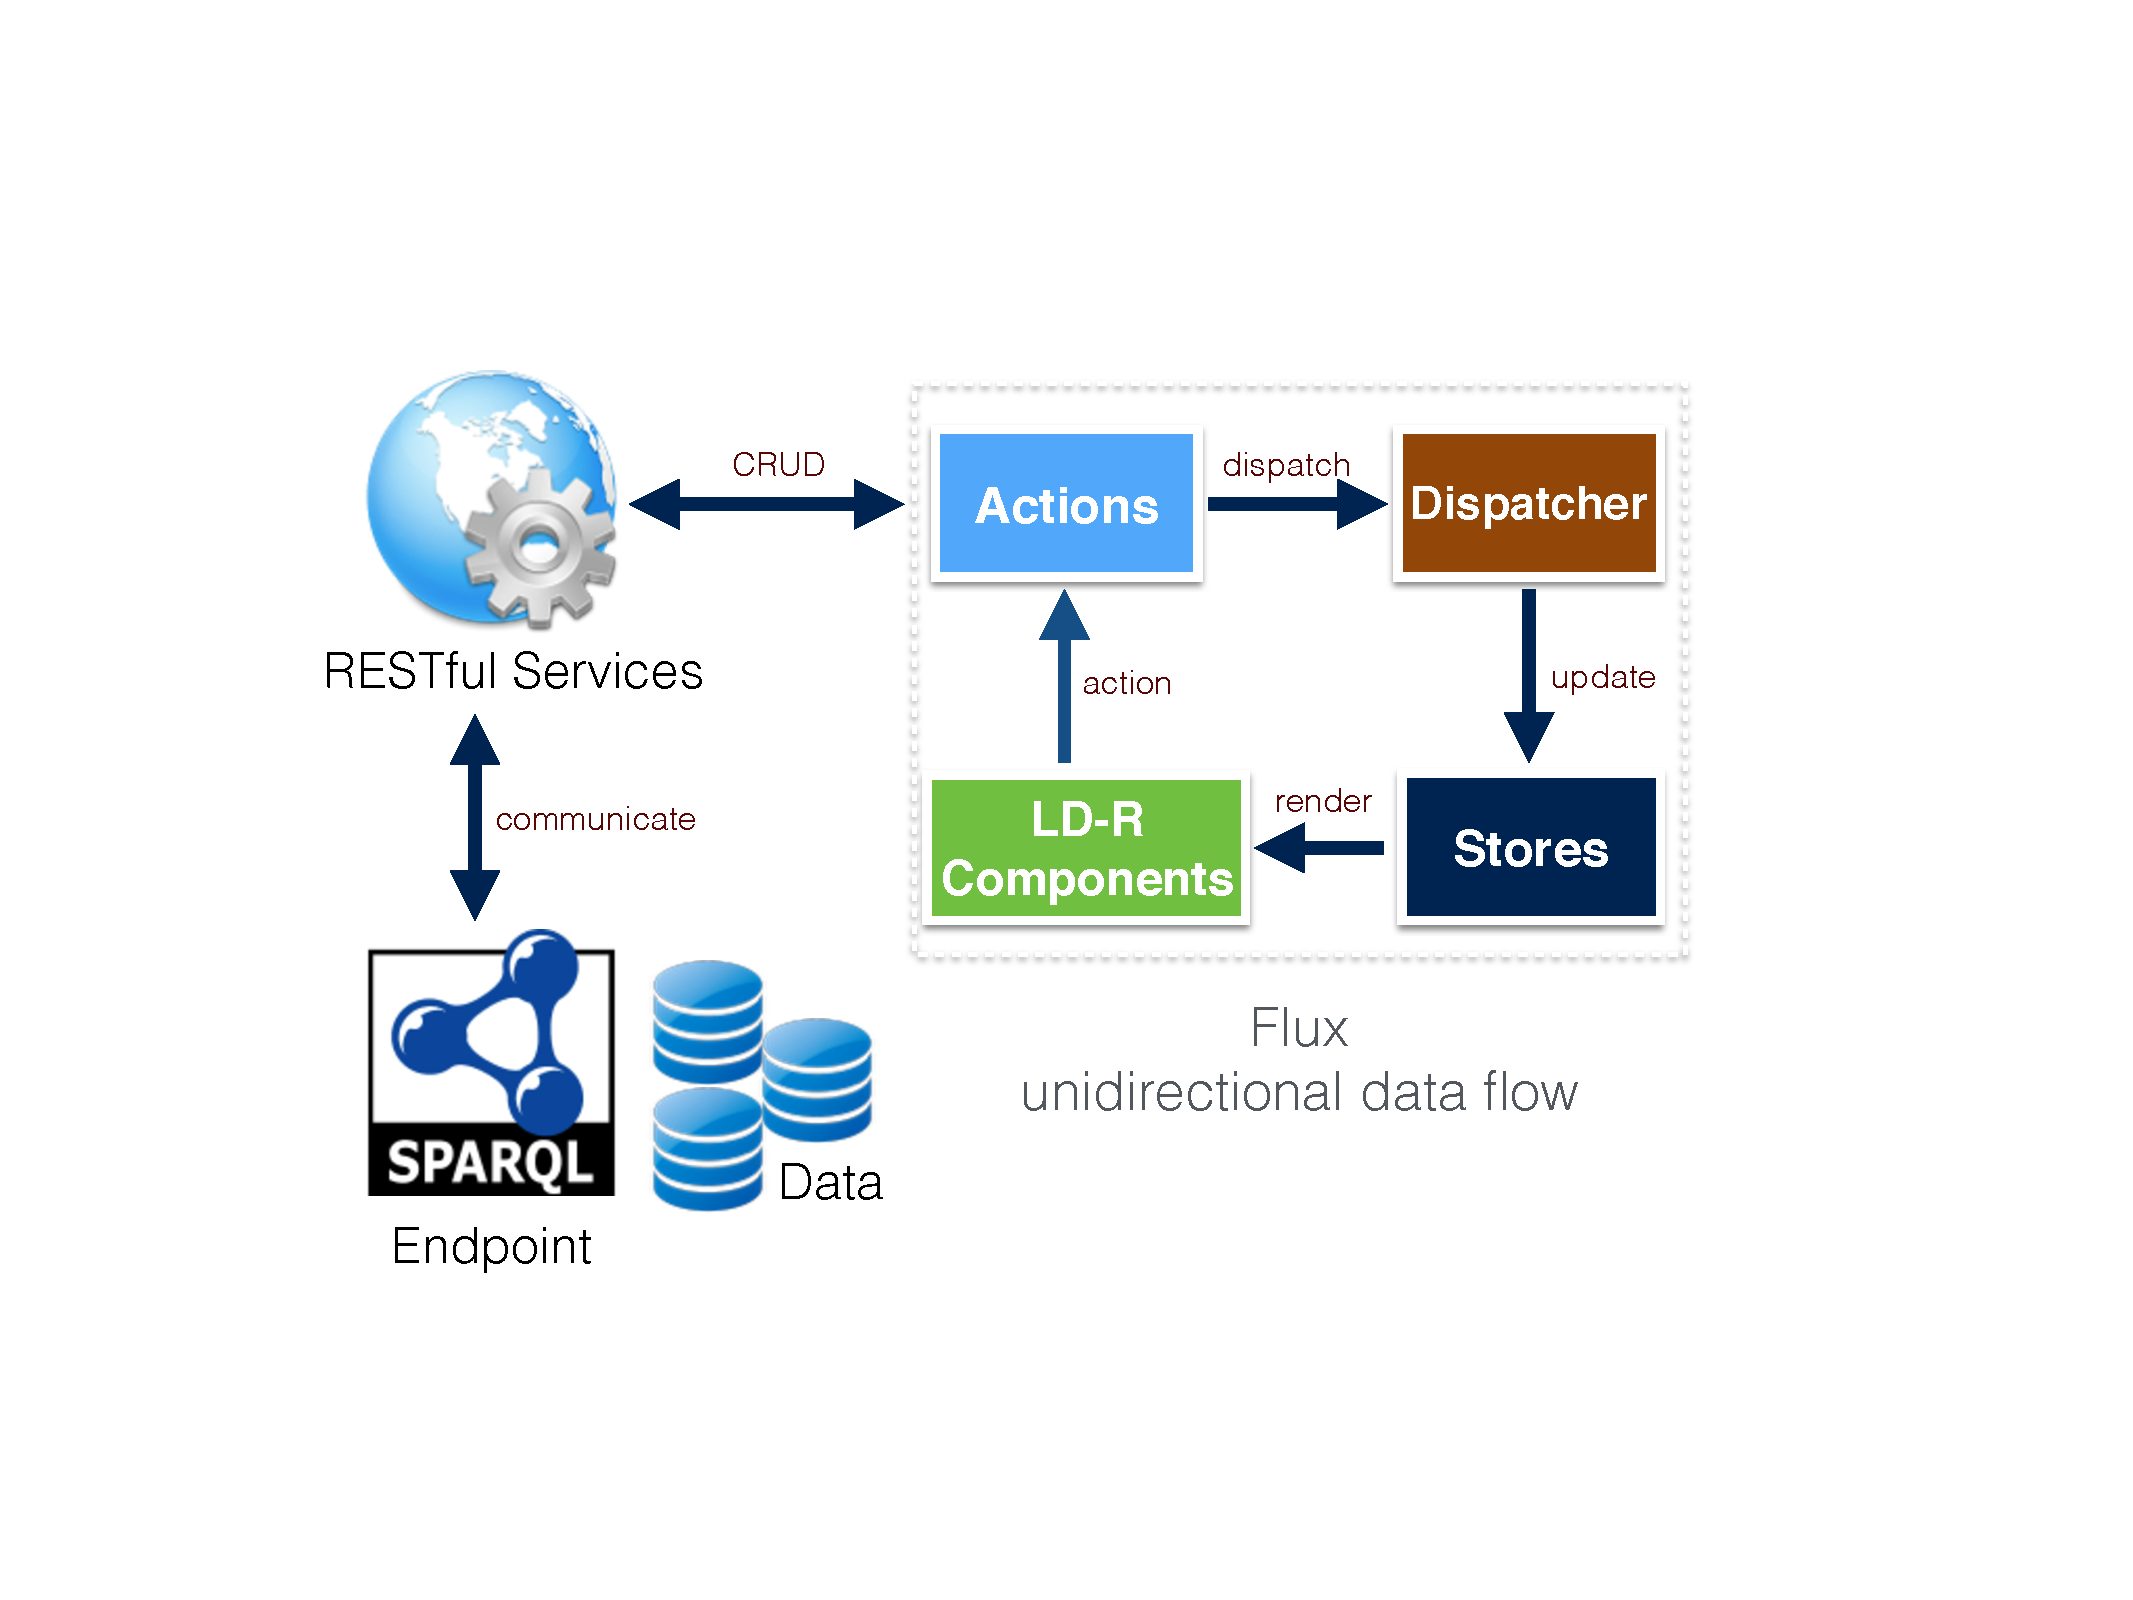
\includegraphics[width=.9\linewidth]{images/dataflow.pdf}
  \caption{Data flow in the LD-Reactor framework.}
  \label{fig:dataflow}
\end{figure}

\section{Implementation}

In order to realize the idea of adaptive Linked Data-driven Web components, we implemented an open-source software framework called \emph{Linked Data Reactor (LD-Reactor)} which is available online at \url{http://ld-r.org}.
LD-Reactor utilizes Facebook's ReactJS\footnote{\url{https://facebook.github.io/react/}} components, the Flux\footnote{\url{https://facebook.github.io/flux}} architecture, Yahoo!'s Fluxible\footnote{\url{http://fluxible.io/}} framework for isomorphic Web applications (i.e. running the components code both on the server and the client) and the Semantic-UI\footnote{\url{http://semantic-ui.com/}} framework for flexible UI themes.
The main reasons we chose \emph{React} components over other  Web Components solutions (e.g. Polymer\footnote{\url{http://www.polymer-project.org/}}, AngularJS\footnote{\url{https://angularjs.org/}}, EmberJS\footnote{\url{http://emberjs.com/}}, etc.) were the maturity and maintainability of the technology, the native multi-platform support, the number of developer tools/components/applications, and the efficiency of its underlying virtual DOM approach\footnote{Elaborating on all these factors is beyond the scope of this paper.}.

As shown in \autoref{fig:dataflow}, LD-Reactor follows the Flux architecture which eschews MVC (Model-View-Controller) in favour of a unidirectional data flow. 
When a user interacts with a React component, the component propagates an action through a central dispatcher, to the various stores that hold the application's data and business logic, and updates all affected components. 
The component interaction with SPARQL endpoints to retrieve and update Linked Data occurs through the invocation of RESTful services in actions.

In order to allow the bootstrapping of LDA UIs, LD-Reactor provides a comprehensive framework that combines the following main elements:
\begin{itemize}

\item A set of RESTful Web services that allow basic CRUD operations on Linked Data using SPARQL queries\footnote{the framework is compliant with the SPARQL 1.1 standard. However, we have identified certain inconsistencies between OpenRDF Sesame and OpenLink Virtuoso RDF stores, which did not allow the execution of syntactically identical queries across both systems. Thereby, specific adaptors have been implemented for each of these two RDF stores.}.

\item A set of core components called \emph{Reactors} which implement core Linked Data components (see \autoref{fig:architecture}) together with their corresponding actions and stores.

\item A set of default components which allow basic viewing, editing and browsing of Linked Data.

\item A set of minimal viable configurations based on the type of data and properties from commonly-used vocabularies on the Semantic Web (e.g. foaf, dcterms and SKOS).

\item A basic access control plugin which allows restricting read/write access to data.

\end{itemize}

%\begin{figure}[htb]
%  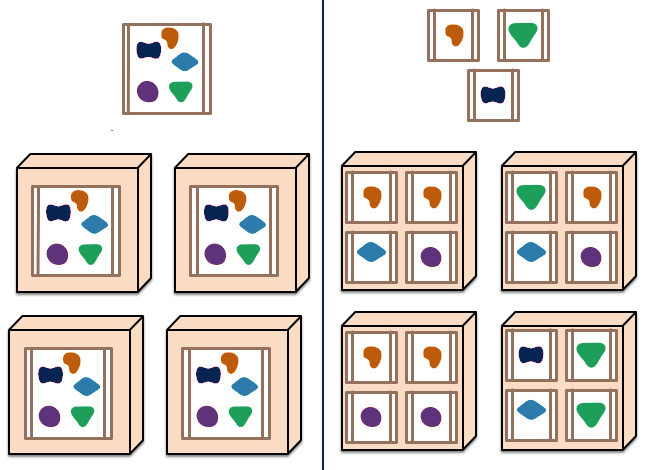
\includegraphics[width=.8\linewidth]{images/microservices.jpg}
%  \caption{Monoliths vs. Microservices~\cite{microservices}}
%  \label{fig:microservices}
%\end{figure}
%

LD-Reactor implementation is compliant with \emph{Microservices Architecture}~\cite{microservices} where the existing ReactJS components can be extended by complementary Linked Data services.
In contrast to the centralized monolithic architecture, the microservices architecture, allows to put the main functionalities of the LDA into separate decoupled services and scale by distributing these services across servers, replicating as needed.
This architectural style also helps to minimize the redeploying of the entire application when changes in components were requested.

%\cite{SmartComposition2015}

\begin{figure}[htb] 
  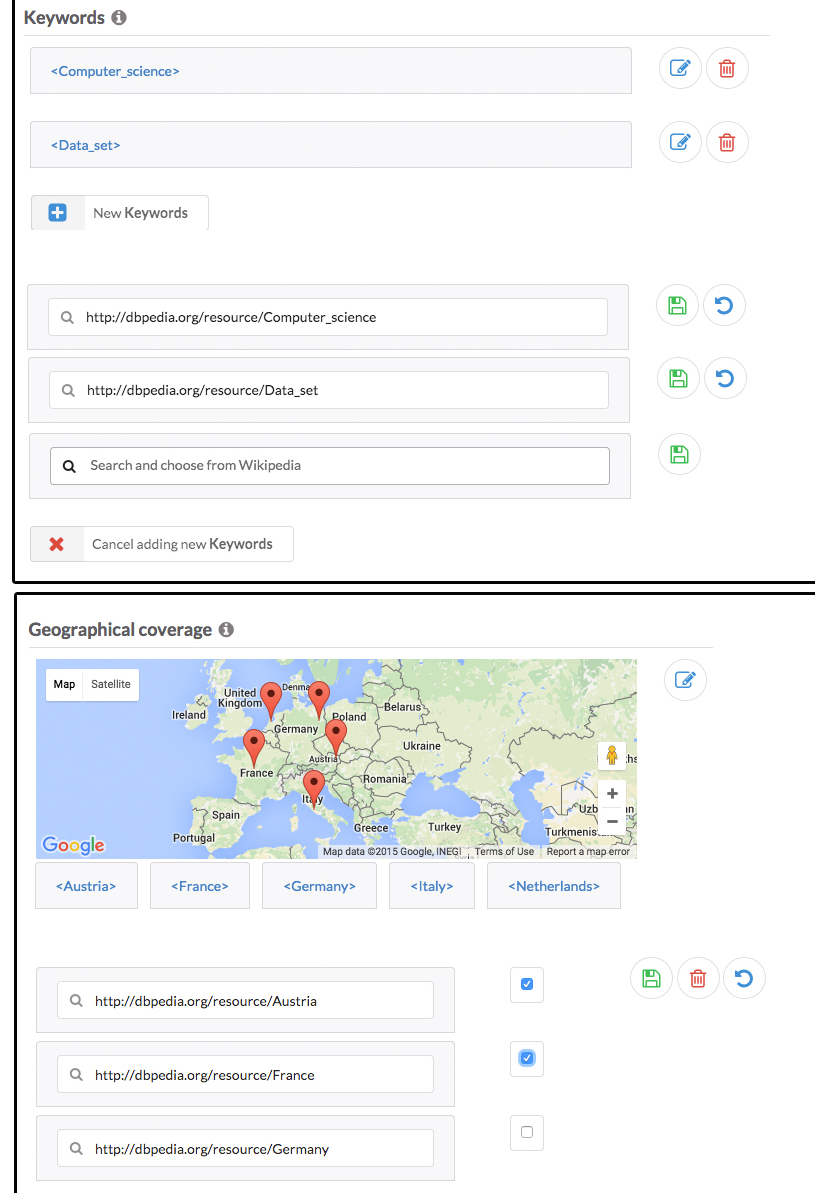
\includegraphics[width=1\linewidth]{images/viewedit.png}
  \caption{A screenshot of LD-Reactor view and edit mode for individual (top) and aggregate (bottom) values.}
  \label{fig:ldrViewEdit}
\end{figure}

\begin{figure}[htb] 
  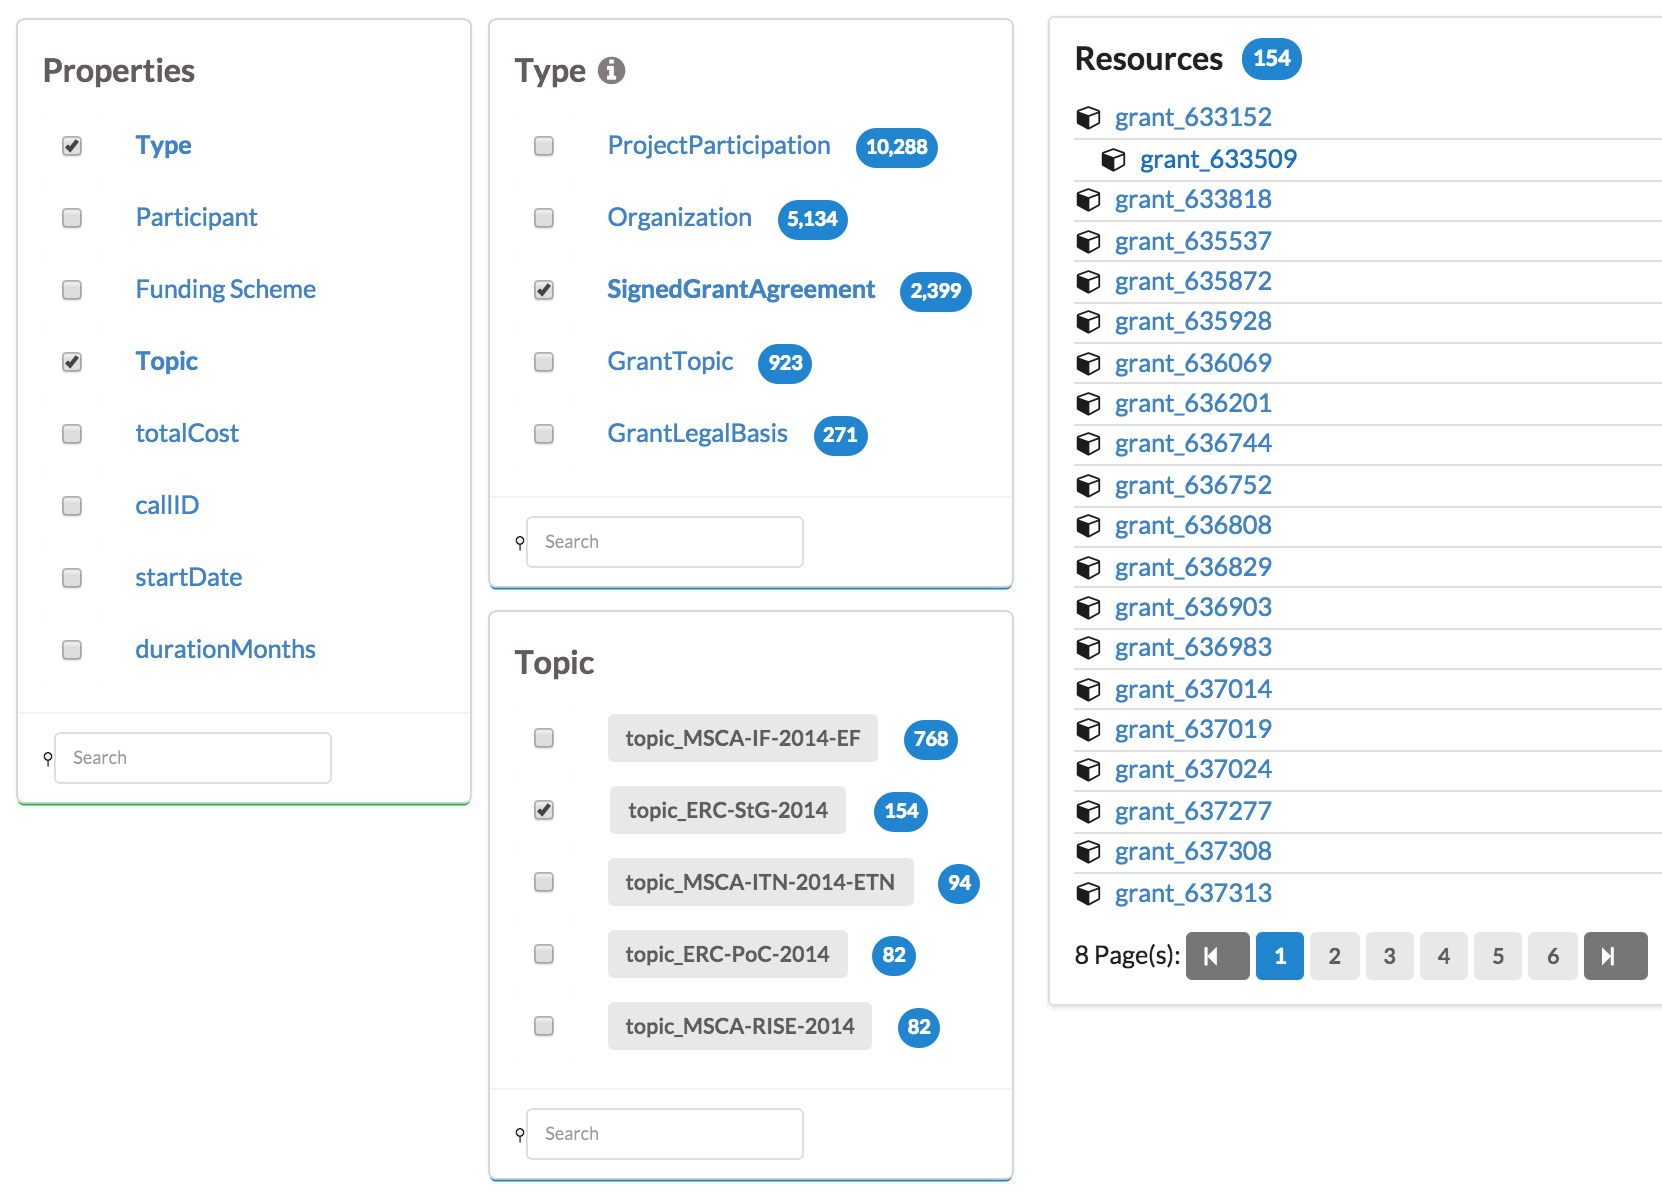
\includegraphics[width=1\linewidth]{images/facets.jpg}
  \caption{A screenshot of LD-Reactor browse mode.}
  \label{fig:ldrBrowse}
\end{figure}

There are three modes of interactions within LD-R components namely \emph{view}, \emph{browse} and \emph{edit} mode.
These modes work with two types of value granularity: individual and aggregate.
As shown in \autoref{fig:ldrViewEdit}, components can target individual values or interact with aggregate values when users want to show/update multiple values at once.
\autoref{fig:ldrBrowse} depicts the browse mode where individual (e.g. item lists with check boxes) and aggregate data browser (e.g. data sliders or maps) components can be employed.

Semantic markup of data (as discussed in Section \ref{sec:markup}) is supported natively within the framework by embedding Microdata annotations within the LD-R Web components.
Additionally, in order to facilitate the creation of component metadata, we developed a tool\footnote{\url{https://github.com/ali1k/ld-r-metadata-generator}} which automatically generates the general metadata about the components in JSON-LD, using \url{Schema.org}'s SoftwareApplication schema\footnote{\url{https://schema.org/SoftwareApplication}}.

\begin{figure*}[ht] 
  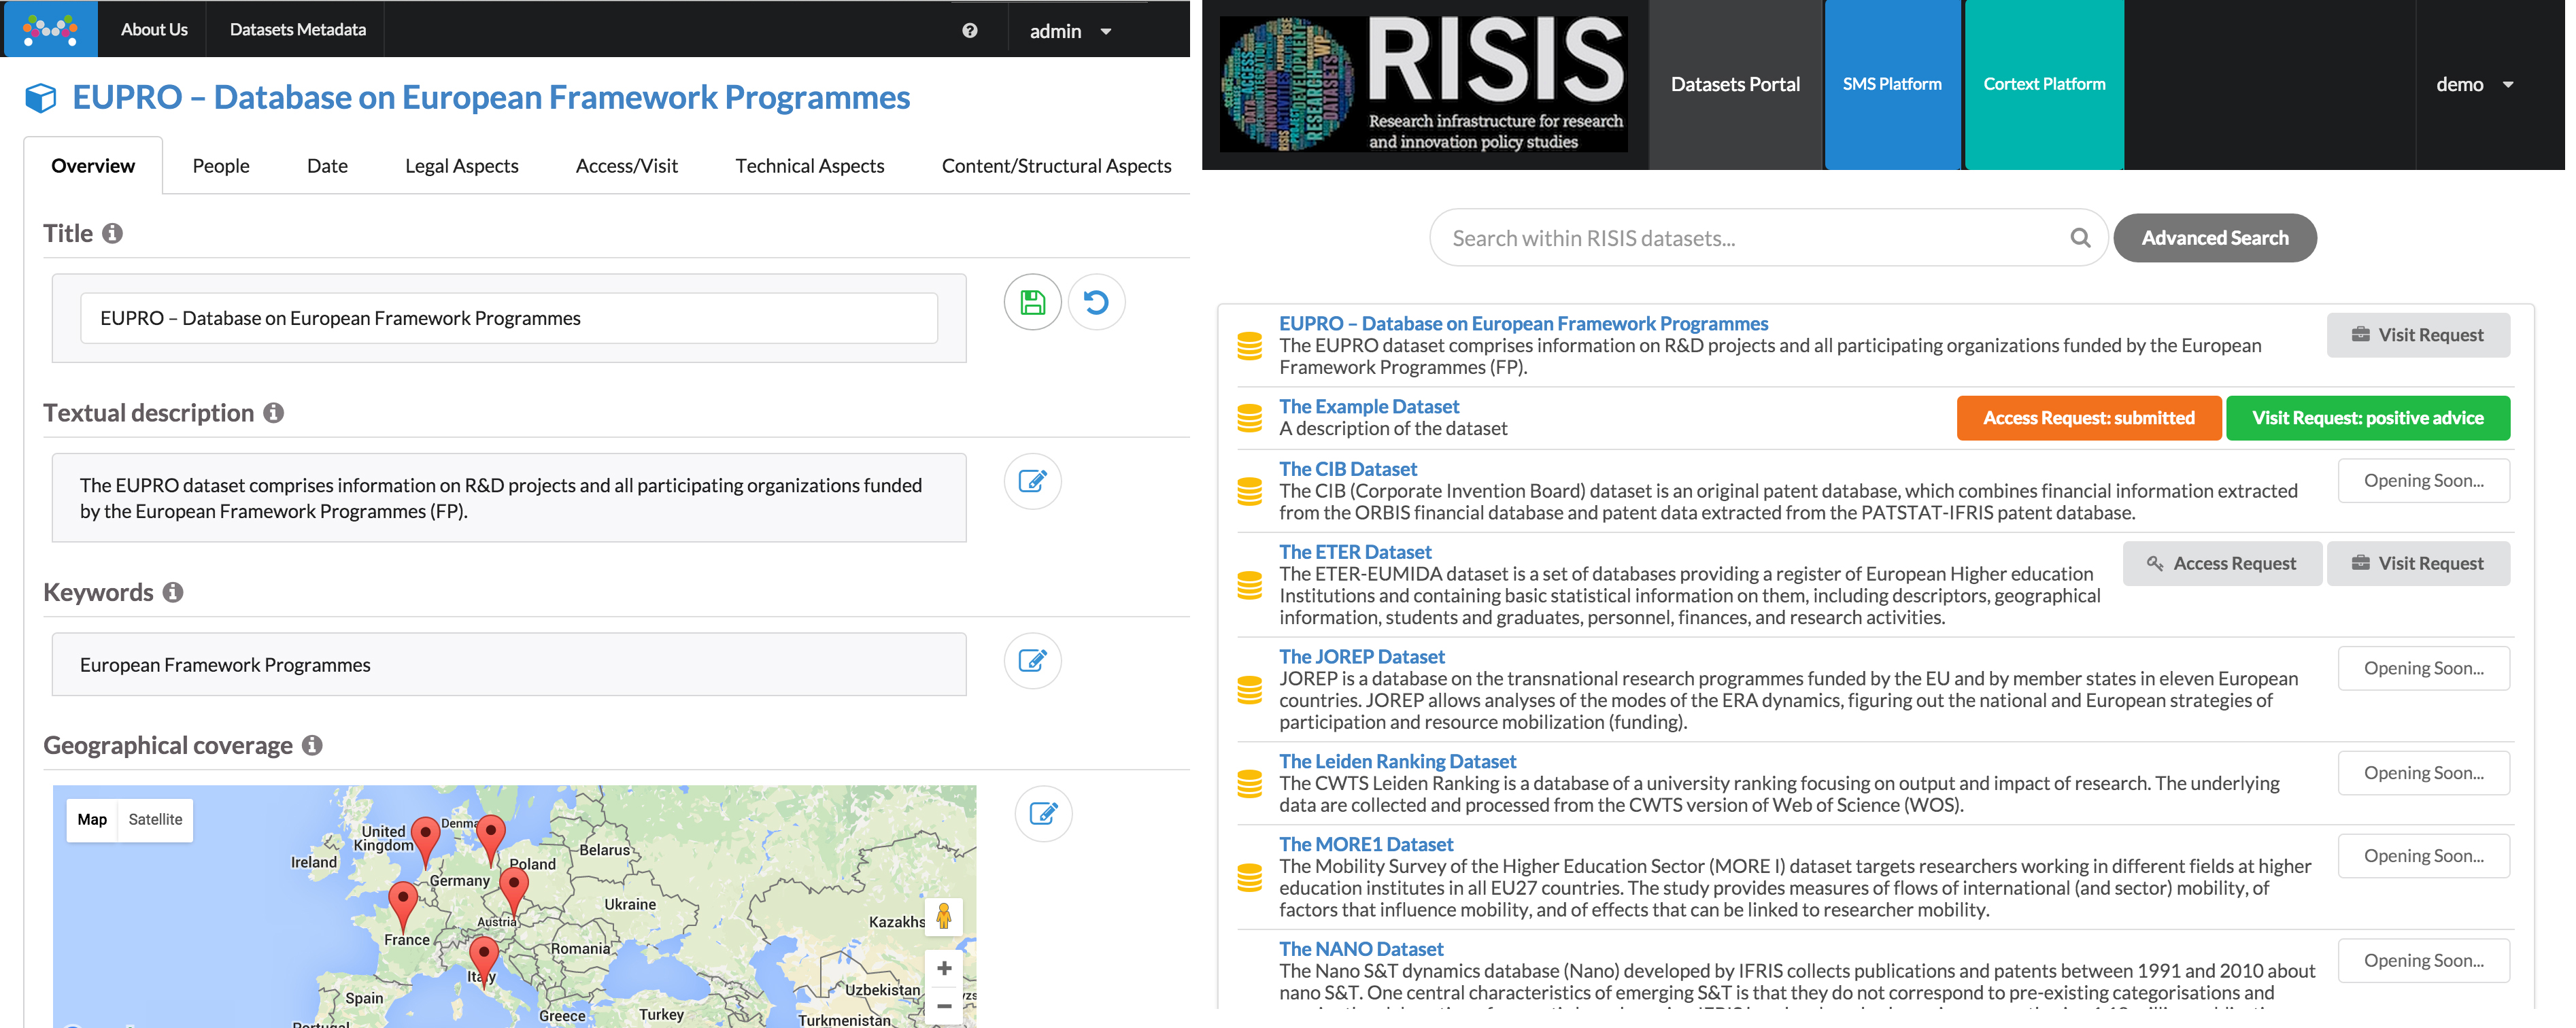
\includegraphics[width=1\linewidth]{images/screenshots.jpg}
  \caption{A screenshot of RISIS metadata editor and datasets portal powered by the LD-Reactor framework.}
  \label{fig:risisScreenshot}
\end{figure*}

\section{Use Cases}

The LD-Reactor framework is already in use within the RISIS\footnote{\url{http://risis.eu}} and Open PHACTS\footnote{\url{http://www.openphacts.org}} projects.

\subsection{RISIS}

The RISIS project aims to provide an infrastructure for research and innovation, targeting researchers from various science and technology domains.
The LD-Reactor frameowrk was utilized in RISIS to help data providers with no Linked Data experience to provide RDF metadata about their datasets\footnote{\url{http://sms.risis.eu}}. This metadata is then used to allow researchers to search the generated metadata to identify and request access to the data they are interested in\footnote{\url{http://datasets.risis.eu}}.
%In order to expose a user-friendly interface to researchers, a set of configurations and components were devised. 
In the following, we present the main requirements for configurations and components, together with their representation in the LD-Reactor configuration file\footnote{see the complete configuration file at \url{http://github.com/risis-eu/sms-platform}}:

\paragraph{Configurations:}
\begin{itemize}
 \item The UI should be able to to render metadata properties in different categories (\autoref{code:config} line 3, 4).
 \item The labels for properties should be changeable in the UI especially for technical properties (e.g. RDF dump) that are unknown to researchers outside the Semantic Web domain (\autoref{code:config} line 18, 26, 40).
 \item There should be a hint for properties to help metadata editors to understand the meaning of the property (\autoref{code:config} line 20, 28, 41).
 \item Instead of showing the full URIs, the output UI should render either a shortened URI or a meaningful string linked to the original URI (\autoref{code:config} line 6). 
 \item Whenever a DBpedia URI is provided, display the corresponding Wikipedia URI in the UI enabling users to retrieve human readable information (\autoref{code:config} line 33, 45).
 \item When a dropdown menu is provided, there should be the ability to accommodate user-defined values which are not listed in the menu (\autoref{code:config} line 57).
 
\end{itemize}

\paragraph{Components:}
\begin{itemize}
 \item A component for \texttt{dcterms:spatial} values to allow searching and inserting resources from DBpedia based on the entity type (e.g. Place, Person, Organization, etc).
 \item A component for \texttt{dcterms:subject} values to allow inserting and viewing DBpedia URIs as subject.
 \item A component for \texttt{dcterms:language} values to allow inserting and viewing languages formatted in ISO 639-1 using standard URIs (e.g. \\ \url{http://id.loc.gov/vocabulary/iso639-1/en}).
 \item A component for \texttt{dcat:byteSize} values to allow inserting and viewing file size specified by a unit.
  \item A component for \texttt{dcterms:format} values to allow inserting and viewing mime types.
\end{itemize}

%\newpage
\begin{lstlisting}[language=json,firstnumber=1, label=code:config, caption=An excerpt of the LD-Reactor configuration for the RISIS metadata editor.]
resource: {
    `generic': {
        usePropertyCategories: 1,
        propertyCategories: [`overview', `legalAspects', `technicalAspects'],
        resourceReactor: [`Resource'],
        shortenURI: 1
    }
},
property: {
    `generic': {
        propertyReactor: [`IndividualProperty'],
        objectReactor: [`IndividualObject'],
        objectIViewer: [`BasicIndividualView'],
        objectIEditor: [`BasicIndividualInput']
    },
    `http://purl.org/dc/terms/language': {
        allowNewValue: 1,
        label: [`Dataset Language'],
        category: [`overview'],
        hint: [`The language of the dataset. Resources defined by the Library of Congress (http://id.loc.gov/vocabulary/iso639-1.html, http://id.loc.gov/vocabulary/iso639-2.html) SHOULD be used.'],
        objectIViewer: [`LanguageView'],
        objectIEditor: [`LanguageInput'],
        defaultValue: [`http://id.loc.gov/vocabulary/iso639-1/en']
    },
    `http://purl.org/dc/terms/spatial': {
         label: [`Geographical coverage'],
         category: [`overview'],
         hint: [`The geographical area covered by the dataset.'],
         allowNewValue: 1,
         objectReactor: [`AggregateObject'],
         objectAViewer: [`DBpediaGoogleMapView'],
         objectIViewer: [`BasicDBpediaView'],
         asWikipedia: 1,
         objectAEditor: [`BasicAggregateInput'],
         objectIEditor: [`DBpediaInput'],
         lookupClass: [`Place']
     },
    `http://purl.org/dc/terms/subject': {
        category: [`overview'],
        label: [`Keywords'],
        hint: [`Tags a dataset with a topic.'],
        allowNewValue: 1,
        objectIEditor: [`DBpediaInput'],
        objectIViewer: [`BasicDBpediaView'],
        asWikipedia: 1
    },
    `http://purl.org/dc/terms/license': {
        category: [`legalAspects'],
        label: [`License'],
        allowNewValue: 1,
        objectIViewer: [`BasicOptionView'],
        objectIEditor: [`BasicOptionInput'],
        options: [
            {label: `Open Data Commons Attribution License', value: `http://www.opendatacommons.org/licenses/by/'},
            {label: `Creative Commons Attribution-ShareAlike', value: `http://creativecommons.org/licenses/by-sa/3.0/'}
        ],
        allowUserDefinedValue: 1
    }   
}
\end{lstlisting}

In accordance to the LD-Reactor microservices architecture (cf. ), we built a \emph{DBpediaGMap} viewer component where we reused the current react-google-maps\footnote{\url{http://github.com/tomchentw/react-google-maps}} together with DBpedia lookup and query services to retrieve the coordinates for the recongnized DBpedia resource values.
\autoref{fig:risisScreenshot} shows a screenshot of the generated UIs for metadata and search.

\subsection{Open PHACTS}

The Open PHACTS Discovery Platform has been developed to reduce barriers to drug discovery, by collecting and integrating a large number of prominent RDF datasets in the pharmacology domain. The platform provides a uniform RESTful API for application developers to access the integrated data.
In collaboration with the data providers, the Open PHACTS consortium has created a comprehensive dataset description specification\footnote{\url{http://www.openphacts.org/specs/2013/WD-datadesc-20130912/}} based on the Vocabulary of Interlinked Datasets (VoID)\footnote{\url{http://www.w3.org/TR/void/}}. The metadata provided in this context enables (among others) exposing the detailed provenance for each result produced by the platform, the location of source files for each dataset, and example resources.

The provision of VoID dataset descriptors that adhere to the specification proved to be a non-trivial challenge, even for data providers that are well versed in providing RDF distributions of their core data. A series of UIs were therefore created to facilitate the creation of the VoID descriptors. However, as the specification evolved over the first 2 years of the project, any changes or additions made had to be reflected in the UI source code as well; a cumbersome process. Due to the inevitable delay between specification changes and UI development, users often found themselves having to edit large RDF files using text editors, which resulted in frequent syntax errors being made.

A new version of the VoID editor implemented using the LD-Reactor framework is now available online\footnote{\url{http://void.ops.labs.vu.nl/} Source: \url{http://github.com/openphacts/ld-r}}. Though the  import/export capabilities of the editor are still not implemented at the time of writing, we have received very positive feedback from the community for a number of reasons:

\begin{figure}[tb] 
  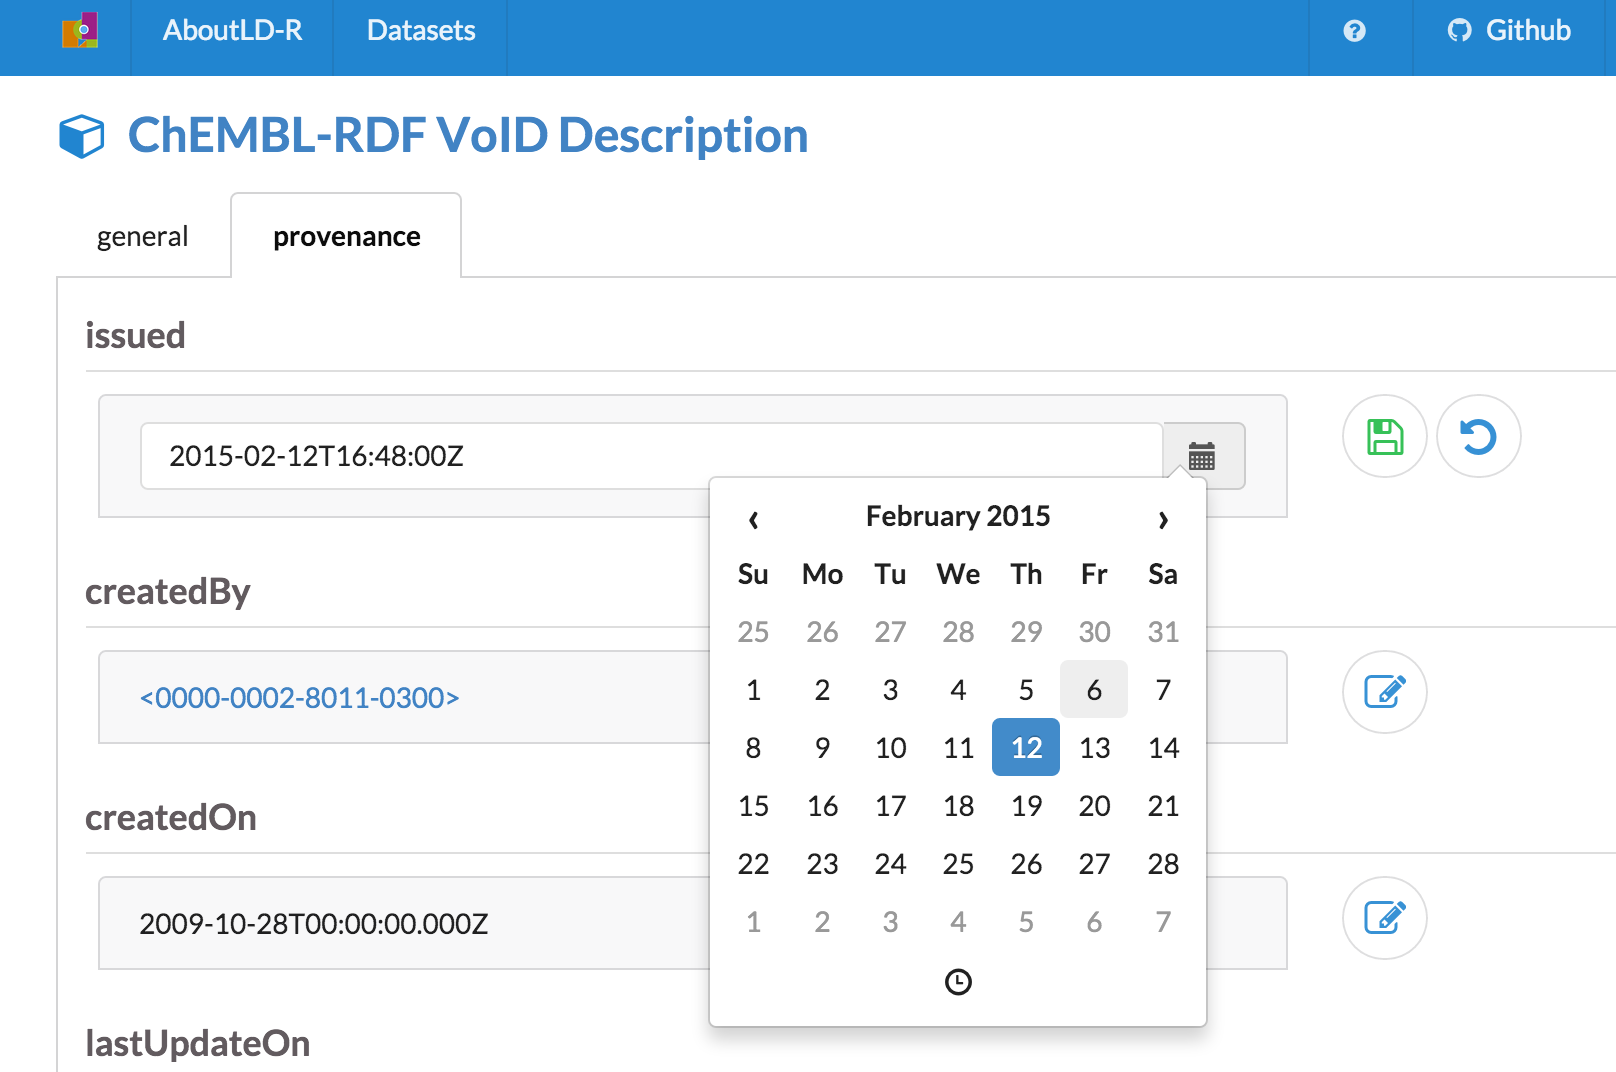
\includegraphics[width=1\linewidth]{images/ops_ldr}
  \caption{A screenshot of the BasicCalendarInput LD-R component created to allow the editing of datetimes in Open PHACTS VoID descriptions.}
  \label{fig:opsLdr}
\end{figure}

\begin{itemize}
	\item UI updates: As the UI is generated based on the underlying data, the process of staying up to date with the current specification becomes trivial. The RDF example provided by the specification can be simply loaded into the RDF store and the changes are immediately visible in the UI through the default core components. Users are then able to adapt the example VoID description to their dataset. The resulting VoID file can be downloaded by exporting all triples in the named graph corresponding to the dataset.
	\item Dataset releases: A large number of property values remain the same across releases. Similarly with using the example from the Dataset Description Specification, users are able to upload their old VoID description and only edit the outdated values.
	\item Access control: Using the built--in user authentication mechanism of LD-Reactor we were able to ensure that only the owner(s) of a particular dataset are able to edit its metadata.
	\item Non-standard properties: Some data providers elect to include additional property that are not prescribed by the specification. The visualisation of such properties is supported easily using the core LD-R components.
	\item Intuitive navigation: Typically, each dataset consists of a number of subsets, which are also of type \texttt{void:Dataset}, and may have further subsets themselves. Displaying all the information together can easily become confusing for the user; instead the LD-Reactor framework was used to provide navigation through the subset links, displaying only a single dataset (or subset) at a time.
	\item Datetime component: Manually typing datetimes in the required format (e.g. `2015-02-12T16:48:00Z') can be an error prone process. Instead, we have been able to reuse the \texttt{react-bootstrap-datetimepicker}\footnote{\url{https://github.com/quri/react-bootstrap-datetimepicker}}, to create a new LD-R value editor for datetimes (BasicCalendarInput) with a graphical interface as shown in \autoref{fig:opsLdr}.
\end{itemize}

In addition to the significant improvements over previous versions of the VoID editor outlined above, we were able to develop the LD-Reactor version in a fraction of the time that was required for earlier versions.

\section{Related Work}
Component-based software engineering (CBSE) has been an active research area since 1987 with numerous results published in the research literature~\cite{Vale2015}.
Within the Semantic Web community, the main focus has been on enriching current service-oriented architectures (SOAs) with semantic formalisms and thereby providing Semantic Web services as reusable and scalable software components~\cite{sws2015}.
There have also been a few attempts to create Semantic Web Components by integrating existing Web-based components with Semantic Web technology~\cite{pahl2011,HartigKF08}.

When it comes to component-based development of LDAs, the works typically fall into 
software application frameworks that address building scalable LDAs in a modular way.
The survey conducted by \cite{SWASurvey09} identified the main issues in current Semantic Web applications and suggested the provision of component-based software frameworks as a potential solution to the identified issues.
The Semantic Web Framework~\cite{swFramework2008} was one of the first attempts in that direction to decompose the LDA development requirements into an architecture of reusable software components.
In most of the current full-stack LDA frameworks such as Callimachus\footnote{\url{http://callimachusproject.org/}} and LDIF\footnote{\url{http://ldif.wbsg.de/}} the focus is mainly on the backend side of LDAs and less attention is paid on how Linked Data is consumed by the end-user. 
There are also more flexible application frameworks such as OntoWiki~\cite{ontowiki-swj} which provide UI widgets and extensions to expose Linked Data to non-Semantic Web end-users.

Besides these generic LDA frameworks, there are also approaches that focus on the development of user interfaces for LDAs.
WYSIWYM (What You See Is What You Mean)~\cite{WYSIWYM2014} is a generic semantics-based UI model to allow integrated visualization, exploration and authoring of structured and unstructured data.
Our proposed approach utilizes the WYSIWYM model for binding RDF-based data to viewer, editor and browser UIs.
Uduvudu~\cite{Uduvudu2015} is another approach to make an adaptive RDF-based UI engine to render Linked Data.
Instead of adopting Web components, Uduvudu employs a set of flexible UI templates that can be combined to create complex UIs. 
Even though the static templates do not provide enough interactions for editing and browsing data (in contrast to Web components), we believe that algorithms for automatic selection of templates employed in Uduvudu can be reused in the LD-Reactor framework for automatic generation of configurations.
Another similar approach is SemwidgJS~\cite{StegemannZ14} which brings a semantic Widget library for the rapid development of LDA UIs.
SemwidgJS offers a simplified query language to allow the navigation of graph-based data by ordinary Web developers.
The main difference between LD-R and SemwidgJS is that LD-Reactor suggests a more interactive model which is not only for displaying Linked Data but also for providing user adaptations based on the meaning of data.
LD-Viewer~\cite{Lukovnikov2014} is another related Linked Data presentation framework particularly tailored for the presentation of DBpedia resources.
In contrast to LD-Reactor, LD-Viewer  builds on top of traditional MVC architecture and its extensions rely heavily on the knowledge of RDF which is a burden for developers unfamiliar with Semantic Web technologies.

In addition to the LDA UI frameworks, there are several ad-hoc tools for Linked Data visualization and exploration such as Balloon Synopsis~\cite{BalloonSchlegelWSGK14} and Sgvizler~\cite{Sgvizler} which can  be utilized as Web components within the LD-Reactor framework. 
\cite{Abascal2015} provides an extensive list of these tools aiming to make Linked Data accessible for common end users who are not familiar with Semantic Web.

Overall, what distinguishes LD-Reactor from the existing frameworks and tools is its modern isomorphic component-based architecture that addresses reactive and reusable UIs as its first class citizen.

\section{Conclusion and Future Work}
This paper presented adaptive Linked Data-driven Web components as a solution to increase the usability of current Linked Data applications.
The proposed component-based solution emphasizes the reusability and separation of concerns in respect to developing Linked Data applications.
The RDF-based UI adaptation mechanism aims to provide better customization and personalization based on the meaning of data.
Furthermore, employing standard Web components aspires to bring a better communication between UX designers and Semantic Web developers in order to reuse best UI practices within Linked Data applications.

As our future plan, we envisage to create a cloud infrastructure to share and reuse LD-R scopes and configurations as well as LD-R Web components without the need to install the framework.
We also plan to make a user interface to facilitate creation of the LD-R scopes and configurations.
Another direction for future research is developing mechanisms for the automatic configuration and composition of Web components based on the semantic markup provided.

\section{Aknowledgement}
We would like to thank our colleagues from the KRR research group at VU University Amsterdam for their helpful comments during the development of the LD-R framework. This work was supported by a grant from the European Union's 7th Framework Programme provided for the project RISIS (GA no. 313082).

\clearpage

\bibliographystyle{abbrv}
\bibliography{refs}

\end{document}
